\section{Mức độ 9,10 điểm}
\setcounter{ex}{0}
\setcounter{dang}{0}
\begin{dang}{Các bài toán thực tế - cực trị}
\end{dang}
\Opensolutionfile{ans}[ans/CD22/Muc_9_10]
\begin{ex}%Câu 1 [2H2K1-4] [Mã 104-2019] 
	Một cơ sở sản xuất có hai bể nước hình trụ có chiều cao bằng nhau, bán kính đáy lần lượt bằng $1\,\,m$ và $1,5\,\,m$. Chủ cơ sở dự định làm một bể nước mới, hình trụ, có cùng chiều cao và thể tích bằng tổng thể tích của hai bể nước trên. Bán kính đáy của bể nước dự định làm gần nhất với kết quả nào dưới đây?
	\choice
	{\True$1,8 m$}
	{$2,1 m$}
	{$1,6 m$}
	{$2,5 m$}
	\loigiai
	{Gọi $h$ là chiều cao của các bể nước và $r$ là bán kính đáy của bể nước dự định làm.\\
		Theo giả thiết, ta có $\pi{r^2}h=\pi{1^2}h+\pi .\left(1,5\right)^2h\Leftrightarrow{r^2}=1+\dfrac{9}{4}=\dfrac{13}{4}.$\\
		Suy ra $r=\dfrac{\sqrt{13}}{2}\approx 1,8.$}
\end{ex}
\begin{ex}%Câu 2 [2H2K1-4] 	[Mã 101 2019]
	Một cơ sở sản xuất có hai bể nước hình trụ có chiều cao bằng nhau, bán kính đáy lần lượt bằng $1\,\,m$ và $1,2\,\,m$. Chủ cơ sở dự định làm một bể nước mới, hình trụ, có cùng chiều cao và có thể tích bằng tổng thể tích của hai bể nước trên. Bán kính đáy của bể nước dự định làm gần nhất với kết quả nào dưới đây?
	\choice
	{$2,2m$}
	{\True$1,6\,m$}
	{$1,8\,m$}
	{$1,4\,m$}
	\loigiai
	{Gọi $R_1;R_2;R$ lần lượt là bán kính của trụ thứ nhất, thứ hai và $h$ là chiều cao của các bể nước.\\ 
		Ta có \\
		$V=V_1+V_2=\pi{R^2}h=\pi{R_1}^2h+\pi{R_2}^2h$
		$\Leftrightarrow {R^2}=R_1^2+R_2^2.$\\ 
		$\Rightarrow R=\sqrt{R_1^2+R_2^2}=\sqrt{1^2+\left(1,2\right)^2}\approx 1,56(m).$\\
		Vậy giá trị cần tìm là $1,56m$.}
\end{ex}
\begin{ex}%Câu 3 [2H2K1-4] 	[Mã 102-2019] 
	Một cơ sở sản xuất có hai bể nước hình trụ có chiều cao bằng nhau, bán kính đáy lần lượt bằng $1\,\,m$ và $1,4\,\,m$. Chủ cơ sở dự định làm một bể nước mới, hình trụ, có cùng chiều cao và có thể tích bằng tổng thể tích của hai bể nước trên. Bán kính đáy của bể nước dự định làm gần nhất với kết quả nào dưới đây?
	\choice
	{\True$1,7\,\,m$}
	{$1,5\,\,m$}
	{$1,9\,\,m$}
	{$2,4\,\,m$}
	\loigiai
	{\begin{center}
			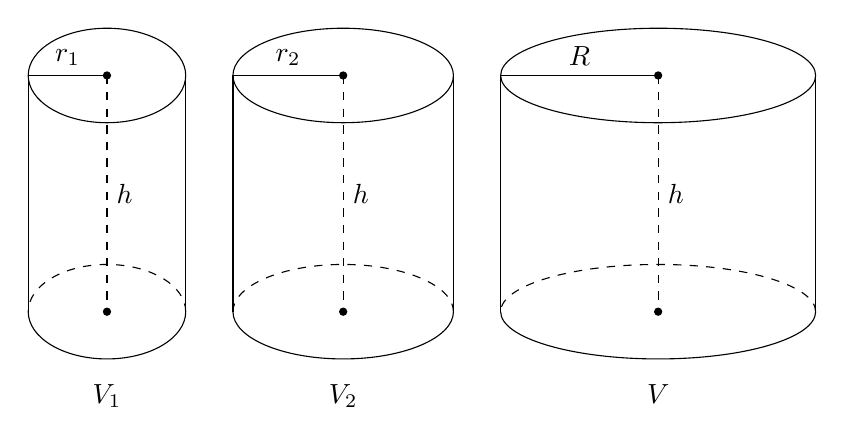
\begin{tikzpicture}
				%	trụ 1
				\draw (0,0) ellipse (1cm and 0.6cm);
				\draw (-1,0) -- (-1,-3);
				\draw (1,0) -- (1,-3);
				\draw (-1,-3) arc (180:360:1cm and 0.6cm);
				\draw[dashed] (1,-3) arc (0:180:1cm and 0.6cm);
				%	trụ 2
				\draw (3,0) ellipse (1.4cm and 0.6cm);
				\draw (1.6,0) -- (1.6,-3);
				\draw (4.4,0) -- (4.4,-3);
				\draw (1.6,-3) arc (180:360:1.4cm and 0.6cm);
				\draw[dashed] (4.4,-3) arc (0:180:1.4cm and 0.6cm);
				%	trụ 3
				\draw (7,0) ellipse (2cm and 0.6cm);
				\draw (5,0) -- (5,-3);
				\draw (9,0) -- (9,-3);
				\draw (5,-3) arc (180:360:2cm and 0.6cm);
				\draw[dashed] (9,-3) arc (0:180:2cm and 0.6cm);
				
				\fill (0,0) circle (1.5pt);
				\fill (0,-3) circle (1.5pt);
				\fill (3,0) circle (1.5pt);
				\fill (3,-3) circle (1.5pt);
				\fill (7,0) circle (1.5pt);
				\fill (7,-3) circle (1.5pt);
				\draw[dashed] (0,0) -- (0,-3) (3,0) -- (3,-3) (7,0) -- (7,-3);
				\node[right] at (0,-1.5) {$h$};
				\node[right] at (3,-1.5) {$h$};
				\node[right] at (7,-1.5) {$h$};
				
				\draw (0,0) -- (-1,0) (1.6,0) -- (3,0) (5,0) -- (7,0);
				\node[above] at (-0.5,0)  {$r_1$};
				\node[above] at (2.3,0)  {$r_2$};
				\node[above] at (6,0)  {$R$};
				
				\node[below] at (0,-3.8) {$V_1$};
				\node[below] at (3,-3.8) {$V_2$};
				\node[below] at (7,-3.8) {$V$};
			\end{tikzpicture}
		\end{center}
		Gọi $r_1;r_2;R$ lần lượt là bán kính của trụ thứ nhất, thứ hai và $h$ là chiều cao của các bể nước.\\
		Ta có: $V=V_1+V_2$ $\Leftrightarrow h\pi{R^2}=h\pi{r_1}^2+h\pi{r_2}^2$.\\
		$\Rightarrow R=\sqrt{r_1^2+r_2^2}\approx 1,72\,m$ .}
\end{ex}
\begin{ex}%Câu 4 [2H2K1-4] 	[Mã 103-2019] 
	Một cơ sở sản xuất có hai bể nước hình trụ có chiều cao bằng nhau, bán kính đáy lần lượt bằng $1\,\,m$ và $1,8\,\,m$. Chủ cơ sở dự định làm một bể nước mới, hình trụ, có cùng chiều cao và có thể tích bằng tổng thể tích của hai bể nước trên. Bán kính đáy của bể nước dự định làm gần nhất với kết quả nào dưới đây?
	\choice
	{$2,8m$}
	{$2,6m$}
	{\True$2,1m$}
	{$2,3m$}
	\loigiai
	{Gọi hai bể nước hình trụ ban đầu lần lượt có chiều cao là $h$, bán kính $r_1,r_2$ và thể tích là $V_1,V_2$.\\
		Ta có một bể nước mới có chiều cao $h$.\\
		Ta có\\ 
		$V=V_1+V_2$.\\
		$\Rightarrow\pi{r^2}h=\pi{r_1}^2h+\pi{r_2}^2h\Rightarrow\pi{r^2}h=\pi{1^2}h+\pi{1,8^2}h\Leftrightarrow r=\sqrt{\dfrac{106}{25}} \approx 2,1m$ .}
\end{ex}
\begin{ex}%Câu 5 [2H2K1-4] 	[Mã 102-2018] 
	Một chiếc bút chì có dạng khối trụ lục giác đều có cạnh đáy $3$ $\left(mm\right)$ và chiều cao bằng $200$ $\left(mm\right)$. Thân bút chì được làm bằng gỗ và phần lõi được làm bằng than chì. Phần lõi có dạng khối trụ có chiều cao bằng chiều cao bằng chiều dài của bút và đáy là hình tròn có bán kính 1 $\left(mm\right)$. Giả định 1 $m^3$ gỗ có giá $a$ triệu đồng, 1 $m^3$ than chì có giá $6a$ triệu đồng. Khi đó giá nguyên vật liệu làm một chiếc bút chì như trên gần nhất với kết quả nào dưới đây?
	\choice
	{$8,45a$ đồng}
	{\True$7,82a$ đồng}
	{$84,5a$ đồng}
	{$78,2a$ đồng}
	\loigiai
	{\begin{center}
			\begin{tikzpicture}[>=stealth, line join=round, line cap=round, font=\footnotesize, scale=1,declare function={a=2;b=a/2;h=4;}]
				\path
				(0,0) coordinate (O)
				foreach \x in {0,...,5}{
					({5+\x*60}:{a} and {b}) coordinate (A\x)
					($(A\x)+(90:h)$) coordinate (B\x)
				}
				;
				\draw (B0)--(B1)--(B2)--(B3)--(B4)--(B5)--cycle
				($(O)+(90:h)$) coordinate (O') ellipse (a and b)
				(O) ellipse (a and b)
				(A0)--(A5)--(A4)--(A3)
				foreach \i in {0,3,4,5}{
					(A\i)--++(90:h)
				}
				(B0)--(B3)
				(B1)--(B4)
				(B2)--(B5)
				(O') circle (a/6 and b/6) 
				;
				\draw[dashed] (A0)--(A1)--(A2)--(A3)
				(A1)--++(90:h)
				(A2)--++(90:h)
				(A0)--(A3)
				(A1)--(A4)
				(A2)--(A5)
				(O) circle (a/6 and b/6)
				(0:a/6 and b/6) --++(90:h)
				(180:a/6 and b/6) --++(90:h)
				;
			\end{tikzpicture}
		\end{center}
		1 $m^3$ gỗ có giá $a$ triệu đồng suy ra một $m{m^3}$ gỗ có giá $\dfrac{a}{1000}$ đồng.\\
		1 $m^3$ than chì có giá $6a$ triệu đồng suy ra $1$ $m{m^3}$ than chì có giá $\dfrac{6a}{1000}$ đồng.\\
		Phần chì của cái bút có thể tích bằng $V_1=200\cdot\pi\cdot{1^2}=200\pi\left(m{m^3}\right)$.\\
		Phần gỗ của của bút chì có thể tích bằng $V_2=200\cdot6\cdot\dfrac{3^2\sqrt{3}}{4}-200\pi=2700\sqrt{3}-200\pi\left(m{m^3}\right)$.\\
		Số tiền làm một chiếc bút chì là $\dfrac{6aV_1+aV_2}{1000}\approx 7,82a$ đồng.}
\end{ex}
\begin{ex}%Câu 6 [2H2K1-4] 	[Mã 101-2018]
	Một chiếc bút chì có dạng khối lăng trụ lục giác đều có cạnh đáy $3mm$ và chiều cao bằng $200mm$. Thân bút chì được làm bằng gỗ và phần lõi được làm bằng than chì. Phần lõi có dạng khối trụ có chiều cao bằng chiều dài của bút và đáy là hình tròn có bán kính đáy $1mm$. Giả định $1$ ${m}^3$ gỗ có giá $a$ (triệu đồng), $1$ ${m}^3$ than chì có giá $8a$ (triệu đồng). Khi đó giá nguyên liệu làm một chiếc bút chì như trên gần nhất với kết quả nào dưới đây?
	\choice
	{$9,07a$ (đồng)}
	{$97,03a$ (đồng)}
	{$90,7a$ (đồng)}
	{\True$9,7a$ (đồng)}
	\loigiai
	{
		Diện tích của khối lăng trụ lục giác đều là $S=6\cdot\left(\left(3.10^{-3}\right)^2\cdot\dfrac{\sqrt{3}}{4}\right)$ (${m}^2$).\\
		Thể tích của chiếc bút chì là: $V=S\cdot h=6\cdot\left(\left(3.10^{-3}\right)^2\cdot\dfrac{\sqrt{3}}{4}\right){200\cdot10^{-3}}=27\sqrt{3}{10^{-7}}$ (${m}^3$).\\
		Thể tích của phần lõi bút chì là $\Delta $ (${m}^3$).\\
		Suy ra thể tích phần thân bút chì là $V_2=V-V_1=\left(27\sqrt{3}-2\pi\right){10^{-7}}$ (${m}^3$).\\
		Giá nguyên liệu làm một chiếc bút chì như trên là:\\
		$V_2\cdot a{10^6}+V_1 \cdot 8a{10^6}$ $=\left(27\sqrt{3}-2\pi\right){10^{-7}}\cdot a{10^6}+2\pi{10^{-7}}\cdot 8a{10^6}$ $=\left(2,7\sqrt{3}+1,4\pi\right)a$ $\simeq 9,07a$ (đồng).}
\end{ex}
%bỏ câu 7

\begin{ex}%Câu 8 [2H2K1-4] 	[Mã 104-2018] 
	Một chiếc bút chì có dạng khối lăng trụ lục giác đều có cạnh đáy $3mm$ và chiều cao $200 mm$. Thân bút chì được làm bằng gỗ và phần lõi được làm bằng than chì. Phần lõi có dạng khối trụ có chiều cao bằng chiều cao của bút và đáy là hình tròn có bán kính 1 $mm$. Giả định $1 {m^3}$ gỗ có giá $a$ (triệu đồng), $1 {m^3}$ than chì có giá $7a$ (triệu đồng). Khi đó giá nguyên vật liệu làm một chiếc bút chì như trên gần nhất với kết quả nào dưới đây?
	\choice
	{$85,5.a$ (đồng)}
	{$9,07.a$ (đồng)}
	{\True$8,45.a$ (đồng)}
	{$90,07.a$ (đồng)}
	\loigiai
	{Thể tích phần lõi than chì: $V_1=\pi\cdot {0,001^2}\cdot 0,2=2\pi{10^{-7}} \text (m^{3})$.\\
		Số tiền làm lõi than chì: $T_1=(2\pi{10^{-7}})\cdot7\cdot a{10^6}=1,4\pi \cdot a$ (đồng).\\
		Thể tích phần thân bằng gỗ của bút:\\
		$V_2=6\cdot \dfrac{(0,003)^2\cdot \sqrt{3}}{4}\cdot 0,2-2\pi{10^{-7}}=\left[\sqrt{3}\cdot{27\cdot10^{-7}}-2\pi{10^{-7}}\right]({m^3})$ .\\
		Số tiền làm phần thân bằng gỗ của bút\\
		$T_2=\left[27\sqrt{3}\cdot{10^{-7}}-\pi{2\cdot10^{-7}}\right]\cdot a\cdot{10^6}=\left[2,7\sqrt{3}-\pi \cdot 0,2\right]\cdot a$ (đồng).\\
		Vậy giá vật liệu làm bút chì là: $T=T_1+T_2\approx 8,45a$ (đồng).
	}
\end{ex}
\begin{ex}%Câu 9 [2H2K1-4] 	[Mã 103-2018]
	Một chiếc bút chì có dạng khối lăng trụ lục giác đều có cạnh đáy bằng $3 mm$ và chiều cao bằng $200mm$. Thân bút chì được làm bằng gỗ và phần lõi có dạng khối trụ có chiều cao bằng chiều dài của bút và đáy là hình tròn có bán kính bằng $1mm$. Giả định $1m^3$ gỗ có giá $a$ (triệu đồng), $1m^3$ than chì có giá $9a$ (triệu đồng). Khi đó giá nguyên vật liệu làm một chiếc bút chì như trên gần nhất với kết quả nào dưới đây?
	\choice
	{$103,3a$ đồng}
	{$97,03a$ đồng}
	{$10,33a$ đồng}
	{\True$9,7a$ đồng}
	\loigiai
	{
		$3mm=0,003m$; $200mm=0,2m$; $1mm=0,001m$\\
		Diện tích đáy của phần than chì: $S_1=\pi{r^2}=\pi\cdot{10^{-6}}(m^2)$.\\
		Diện tích đáy phần bút bằng gỗ:\\ $S_2=6S_{OAB}-S_1=\left(6\cdot \dfrac{3^2\sqrt{3}}{4}-\pi\right){10^{-6}}=\left(\dfrac{27\sqrt{3}}{2}-\pi\right)\cdot{10^{-6}}(m^2)$.\\
		Thể tích than chì cần dùng: $V_1=S_1\cdot h=\pi\cdot{r^2}\cdot0,2=0,2\cdot \pi\cdot{10^{-6}}(m^3)$.\\
		Thể tích gỗ làm bút chì: $V_2=S_2\cdot h=\left(\dfrac{27\sqrt{3}}{2}-\pi\right){0,2\cdot 10^{-6}}(m^3)$.\\
		Tiền làm một cây bút:\\ $V_1\cdot9a+V_2\cdot a=\left(9V_1+V_2\right)a=\left(9\cdot0,2\pi{10^{-6}}+\left(\dfrac{27\sqrt{3}}{2}-\pi\right){0,2\cdot10^{-6}}\right) a=9,7 a$ (đồng).}
\end{ex}
%%%---10-17---
\begin{ex}%Câu 10 [2H2B1-4]	[Chuyên Lê Quý Đôn Quảng Trị 2019] 
	Người ta làm tạ tập cơ tay như hình vẽ với hai đầu là hai khối trụ bằng nhau và tay cầm cũng là khối trụ. Biết hai đầu là hai khối trụ đường kính đáy bằng $12$, chiều cao bằng $6$, chiều dài tạ bằng $30$ và bán kính tay cầm là $2$. Hãy tính thể tích vật liệu làm nên tạ tay đó.
	\begin{center}
		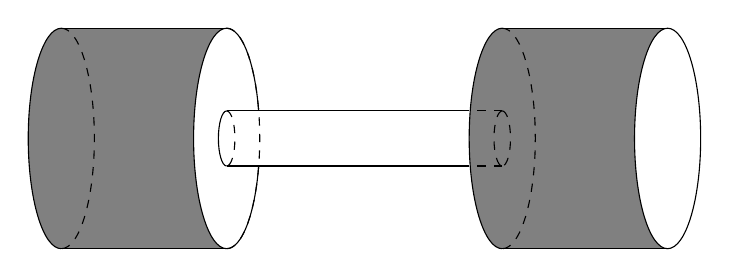
\begin{tikzpicture}[scale=.7]
			\fill[gray,smooth] (0,2) -- (3,2) -- (3,2) arc (90:270:0.6cm and 2cm) -- (0,-2) -- (0,-2) arc (-90:-270:0.6cm and 2cm) -- cycle;
			\fill[gray,smooth] (8,2) -- (11,2) -- (11,2) arc (90:270:0.6cm and 2cm) -- (8,-2) -- (8,-2) arc (-90:-270:0.6cm and 2cm) -- cycle;
			%			Đầu tạ
			\draw (0,2) arc (90:270:0.6cm and 2cm);
			\draw[dashed] (0,2) arc (90:-90:0.6cm and 2cm);
			\draw (0,2) -- (3,2) (8,2) -- (11,2) (0,-2) -- (3,-2) (8,-2) -- (11,-2);
			\draw (3,2) arc (90:270:0.6cm and 2cm);
			\draw (3,2) arc (90:15:0.6cm and 2cm);
			\draw (3,-2) arc (-90:-15:0.6cm and 2cm);
			\draw[dashed] (3,2) arc (90:-90:0.6cm and 2cm);
			\draw (8,2) arc (90:270:0.6cm and 2cm);
			\draw[dashed] (8,2) arc (90:-90:0.6cm and 2cm);
			\draw (11,0) ellipse (0.6cm and 2cm);
			%		  Tay cầm
			\draw (3,0.5) arc (90:270:0.15cm and 0.5cm);
			\draw[dashed] (3,0.5) arc (90:-90:0.15cm and 0.5cm);
			\draw[dashed] (8,0.5) arc (90:270:0.15cm and 0.5cm);
			\draw[dashed] (8,0.5) arc (90:-90:0.15cm and 0.5cm);
			\draw (3,0.5) -- (7.4,0.5) (3,-0.5) -- (7.4,-0.5);
			\draw[dashed] (8,0.5) -- (7.4,0.5) (8,-0.5) -- (7.4,-0.5);
		\end{tikzpicture}
	\end{center}
	\choice
	{$108\pi $}
	{$6480\pi $}
	{$502\pi $}
	{\True $504\pi $}
	\loigiai{
		Gọi $h_1$, $R_1$, $V_1$ lần lượt là chiều cao, bán kính đáy, thể tích khối trụ nhỏ mỗi đầu.\\
		$V_1=h_1\cdot \pi \cdot R_1^2=6\cdot\pi \cdot6^2=216\pi $.\\
		Gọi $h_2$, $R_2$, $V_2$ lần lượt là chiều cao, bán kính đáy, thể tích của tay cầm.\\
		$V_2=h_2\cdot \pi \cdot R_2^2=\left(30-2\cdot 6\right)\cdot \pi \cdot 2^2=72\pi $.\\
		Thể tích vật liệu làm nên tạ tay bằng $V=2V_1+V_2=504\pi $.}
\end{ex}

\begin{ex}%Câu 11 [2H2K1-4]	[THPT Lê Quý Đôn - Điện Biên 2019] 
	Một người thợ có một khối đá hình trụ. Kẻ hai đường kính $MN$, $PQ$ của hai đáy sao cho $MN\perp PQ$. Người thợ đó cắt khối đá theo các mặt đi qua $3$ trong $4$ điểm $M$, $N$, $P$, $Q$ để khối đá có hình tứ diện $MNPQ$. Biết $MN=60$ cm và thể tích khối tứ diện $MNPQ=30$ $\mathrm{\,d}{\text{m}^3}$. Hãy tính thể tích lượng đá cắt bỏ (làm tròn đến một chữ số thập phân sau dấu phẩy).
	\choice
	{$101,3\mathrm{\,d}{\text{m}^3}$}
	{\True $111,4\mathrm{\,d}{\text{m}^3}$}
	{$121,3\mathrm{\,d}{\text{m}^3}$}
	{$141,3\mathrm{\,d}{\text{m}^3}$}
	\loigiai
	{\begin{center}
			\begin{tikzpicture}
				\draw (0,0) ellipse (2cm and 0.6cm);
				\draw (-2,0) -- (-2,-4);
				\draw (2,0) -- (2,-4);
				\draw (-2,-4) arc (180:360:2cm and 0.6cm);
				\draw[dashed] (2,-4) arc (0:180:2cm and 0.6cm);
				\fill (0,0) circle (1.5pt);
				\fill (0,-4) circle (1.5pt);
				\node[draw,fill,circle,inner sep=1pt,label={180:$M$}] (M) at (180:2cm and 0.6cm) {};
				\node[draw,fill,circle,inner sep=1pt,label={0:$N$}] (N) at (0:2cm and 0.6cm) {};
				\node[draw,fill,circle,inner sep=1pt,label={-90:$P$}] (P) at ($(0,-4)+(-60:2 and 0.6)$) {};
				\node[draw,fill,circle,inner sep=1pt,label={-90:$Q$}] (Q) at ($(0,-4)+(120:2 and 0.6)$) {};
				\draw[dashed] (N) -- (Q) -- (P) -- (M) -- (Q);
				\node[above] at (0,0) {$O$};
				\node[below] at (0,-4) {$O'$};
				\draw (M) -- (N) -- (P);
			\end{tikzpicture}
		\end{center}
		Gọi $O$ và $O'$ lần lượt là trung điểm $MN$ và $PQ$.\\
		Khi đó $OO'$ là trục của hình trụ và $O{O}'\perp MN\Rightarrow MN\perp\left(OPQ\right)$.\\
		$V_{MNPQ}=\dfrac{1}{3}MN\cdot S_{OPQ}=\dfrac{O{O}'\cdot {6^2}}{6}=6\cdot O{O}'$ $\left(\mathrm{\,d}{\text{m}^{\text{3}}}\right)$.\\
		Theo bài ra ta có $V_{MNPQ}=30$ $\mathrm{\,d}{\text{m}^3}\Rightarrow O{O}'=5$ $\text{dm}$.\\
		Thể tích khối trụ là $V_\text{trụ}=\pi\cdot {3^2}\cdot 5\approx 141,4$ $\mathrm{\,d}{\text{m}^3}$.\\
		Vậy thể tích lượng đá cắt bỏ $V=V_\text{trụ}-V_{MNPQ}\approx 111,4$ $\mathrm{\,d}{\text{m}^3}$.}
\end{ex}

\begin{ex}%Câu 12 [2H2G1-5]	[Chuyên Trần Phú Hải Phòng 2019] 
	Công ty $X$ định làm một téc nước hình trụ bằng inox (gồm cả nắp) có dung tích $1$ m$^3$. Để tiết kiệm chi phí công ty $X$ chọn loại téc nước có diện tích toàn phần nhỏ nhất. Hỏi diện tích toàn phần của téc nước nhỏ nhất bằng bao nhiêu (kết quả làm tròn đến $2$ chữ số sau dấu phẩy)?
	\choice
	{$5,59$ m$^2$}
	{\True $5,54$ m$^2$}
	{$5,57$ m$^2$}
	{$5,52$ m$^2$}
	\loigiai{
		Ta có: $V=\pi{R^2}h=1\Rightarrow\left\{\begin{aligned}
			&\pi Rh=\dfrac{1}{R}\\ 
			&\pi{R^2}=\dfrac{1}{h}\\ 
		\end{aligned}\right.$\\
		Diện tích toàn phần của téc nước: $S_{tp}=2\pi Rh+2\pi{R^2}=\dfrac{2}{R}+2\pi{R^2}$.\\
		Xét $S'=4\pi R-\dfrac{2}{R^2}=0\Leftrightarrow R=\sqrt[3]{\dfrac{1}{2\pi}}$.\\
		\begin{center}
			
\begin{tikzpicture}
				\tkzTabInit
				[lgt=3,espcl=5] % tùy chọn
				{$R$/1.2, $S'$/1, $S_{tp}$/2.5}
				{0, $\sqrt[3]{\dfrac{1}{2\pi}}$, $+\infty$}
				\tkzTabLine{,-,0,+,} % hàng 2 cột 2
				\tkzTabVar{+/ $+\infty$, -/ $-\dfrac{\Delta}{4a}$, +/ $+\infty$} % hàng 3 cột 2
			\end{tikzpicture}
		\end{center}
		Từ bảng biến thiên ta có $S_{tp}$ đạt giá trị nhỏ nhất tại $R=\sqrt[3]{\dfrac{1}{2\pi}}$.\\
		$\Rightarrow{S_{\left(tp\right)\min}}=2\sqrt[3]{2\pi}+\dfrac{2\pi}{\sqrt[3]{4\pi^2}}\approx 5,54$.}
\end{ex}

\begin{ex}%Câu 13 [2H2B1-4]	[Trường VINSCHOOL-2020] 
	Một chiếc tạ tay có hình dạng gồm 3 khối trụ, trong đó hai khối trụ ở hai đầu bằng nhau và khối trụ làm tay cầm ở giữa. Gọi khối trụ làm đầu tạ là $\left(T_1\right)$ và khối trụ làm tay cầm là $\left(T_2\right)$ lần lượt có bán kính và chiều cao tương ứng là $r_1$, $h_1$, $r_2$, $h_2$ thỏa mãn $r_1=4r_2$, $h_1=\dfrac{1}{2}{h_2}$ (tham khảo hình vẽ).
	\begin{center}
		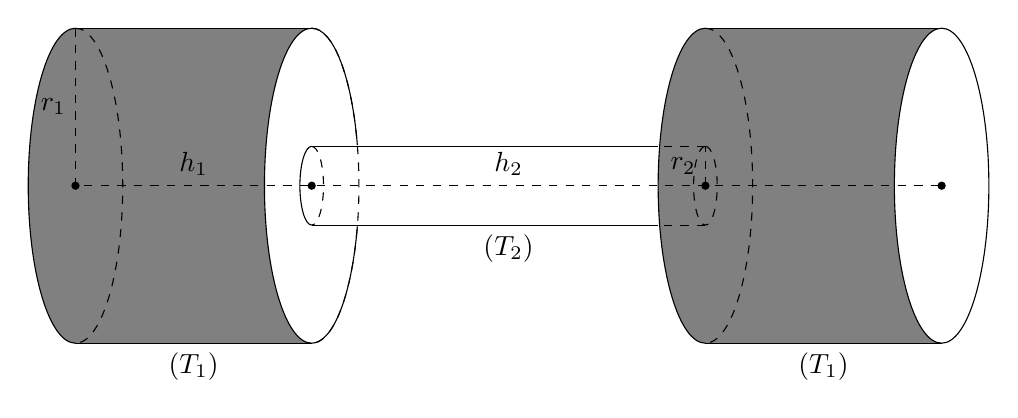
\begin{tikzpicture}
			\fill[gray,smooth] (0,2) -- (3,2) -- (3,2) arc (90:270:0.6cm and 2cm) -- (0,-2) -- (0,-2) arc (-90:-270:0.6cm and 2cm) -- cycle;
			\fill[gray,smooth] (8,2) -- (11,2) -- (11,2) arc (90:270:0.6cm and 2cm) -- (8,-2) -- (8,-2) arc (-90:-270:0.6cm and 2cm) -- cycle;
			%			Đầu tạ
			\draw (0,2) arc (90:270:0.6cm and 2cm);
			\draw[dashed] (0,2) arc (90:-90:0.6cm and 2cm);
			\draw (0,2) -- (3,2) (8,2) -- (11,2) (0,-2) -- (3,-2) (8,-2) -- (11,-2);
			\draw (3,2) arc (90:270:0.6cm and 2cm);
			\draw (3,2) arc (90:15:0.6cm and 2cm);
			\draw (3,-2) arc (-90:-15:0.6cm and 2cm);
			\draw[dashed] (3,2) arc (90:-90:0.6cm and 2cm);
			\draw (8,2) arc (90:270:0.6cm and 2cm);
			\draw[dashed] (8,2) arc (90:-90:0.6cm and 2cm);
			\draw (11,0) ellipse (0.6cm and 2cm);
			%		  Tay cầm
			\draw (3,0.5) arc (90:270:0.15cm and 0.5cm);
			\draw[dashed] (3,0.5) arc (90:-90:0.15cm and 0.5cm);
			\draw[dashed] (8,0.5) arc (90:270:0.15cm and 0.5cm);
			\draw[dashed] (8,0.5) arc (90:-90:0.15cm and 0.5cm);
			\draw (3,0.5) -- (7.4,0.5) (3,-0.5) -- (7.4,-0.5);
			\draw[dashed] (8,0.5) -- (7.4,0.5) (8,-0.5) -- (7.4,-0.5) (0,2) -- (0,0) -- (11,0) (8,0) -- (8,0.5);
			\fill (0,0) circle (1.5pt);
			\fill (3,0) circle (1.5pt);
			\fill (8,0) circle (1.5pt);
			\fill (11,0) circle (1.5pt);
			\node[above] at (1.5,0) {$h_1$};
			\node[above] at (5.5,0) {$h_2$};
			\node[left] at (0,1) {$r_1$};
			\node[left] at (8,0.25) {$r_2$};
			\node[below] at (1.5,-2) {$(T_1)$};
			\node[below] at (9.5,-2) {$(T_1)$};
			\node[below] at (5.5,-0.5) {$(T_2)$};
		\end{tikzpicture}
	\end{center}
	Biết rằng thể tích của khối trụ tay cầm $\left(T_2\right)$ bằng 30 (cm$^3$) và chiếc tạ làm bằng inox có khối lượng riêng là $D=7,7$ g/cm$^3$. Khối lượng của chiếc tạ tay bằng
	\choice
	{\True $3,927$ kg}
	{$2,927$ kg}
	{$3,279$ kg}
	{$2,279$ kg}
	\loigiai
	{
		Thể tích của hai khối trụ làm đầu tạ $\left(T_1\right)$ : $V_1=2\pi  r_1^2h_1=2\pi{\left(4r_2\right)^2}\dfrac{1}{2}{h_2}=16\pi r_2^2h_2=16\cdot 30=480$ (cm$^3$).\\
		Tổng thể tích của chiếc tạ tay là $V=V_1+V_2=480+30=510$ (cm$^3$).\\
		Khối lượng của chiếc tạ là $m=D\cdot V=7,7\cdot 510=3927$ (g) $=3,927$ (kg).}
\end{ex}

\begin{ex}%Câu 14 [2H2K1-4]	[Thi thử hội 8 trường chuyên 2019] 
	Một công ty sản xuất bút chì có dạng hình lăng trụ lục giác đều có chiều cao $18$ $\text{cm}$ và đáy là hình lục giác nội tiếp đường tròn đường kính $1\operatorname{cm}$. Bút chì được cấu tạo từ hai thành phần chính là than chì và bột gỗ ép, than chì là một khối trụ ở trung tâm có đường kính $\dfrac{1}{4}$ $\text{cm}$, giá thành $540$ đồng$/{\operatorname{cm}^3}$. Bột gỗ ép xung quanh có giá thành $100$ đồng$/{\operatorname{cm}^3}$. Tính giá của một cái bút chì được công ty bán ra biết giá nguyên vật liệu chiếm $15,58\%$ giá thành sản phẩm.
	\choice
	{\True $10000$ đồng}
	{$8000$ đồng}
	{$5000$ đồng}
	{$3000$ đồng}
	\loigiai{
		\begin{center}
			\begin{tikzpicture}[>=stealth, line join=round, line cap=round, font=\footnotesize, scale=1,declare function={a=2;b=a/2;h=4;}]
				\path
				(0,0) coordinate (O)
				foreach \x in {0,...,5}{
					({5+\x*60}:{a} and {b}) coordinate (A\x)
					($(A\x)+(90:h)$) coordinate (B\x)
				}
				;
				\draw (B0)--(B1)--(B2)--(B3)--(B4)--(B5)--cycle
				($(O)+(90:h)$) coordinate (O') %ellipse (a and b)
				%				(O) ellipse (a and b)
				(A0)--(A5)--(A4)--(A3)
				foreach \i in {0,3,4,5}{
					(A\i)--++(90:h)
				}
				(O') circle (a/3 and b/3) 
				;
				\draw[dashed] (A0)--(A1)--(A2)--(A3)
				(A1)--++(90:h)
				(A2)--++(90:h)
				(O) circle (a/3 and b/3)
				(0:a/3 and b/3) --++(90:h)
				(180:a/3 and b/3) --++(90:h)
				;
			\end{tikzpicture}
		\end{center}
		Gọi $R$ và $r$ lần lượt là bán kính đường tròn ngoại tiếp lục giác đều và bán kính của lõi than chì.\\
		Ta có $R=\dfrac{1}{2}\operatorname{cm}$ và $r=\dfrac{1}{8}\operatorname{cm}$.\\
		Suy ra diện tích của lục giác đều là $S=6\cdot R^2\cdot \dfrac{\sqrt{3}}{4}=6\cdot \dfrac{1}{4}\cdot \dfrac{\sqrt{3}}{4}=\dfrac{3\sqrt{3}}{8}$.\\
		Gọi $V$ là thể tích của khối lăng trụ lục giác đều. $V_1$, $V_2$ lần lượt là thể tích của khối than chì và bột gỗ dùng để làm ra một cây bút chì.\\
		Ta có $V=S\cdot h=\dfrac{3\sqrt{3}}{8}\cdot 18=\dfrac{27\sqrt{3}}{4}\left(\operatorname{cm}^3\right)$; $V_1=\pi{r^2}h=\pi\cdot \dfrac{1}{8^2}\cdot 18=\dfrac{9\pi}{32}\left(\operatorname{cm}^3\right)$.\\
		$\Rightarrow{V_2}=V-V_1=\dfrac{27\sqrt{3}}{4}-\dfrac{9\pi}{32}\left(\operatorname{cm}^3\right)$.\\
		Do đó, giá nguyên vật liệu dùng để làm một cây bút chì là $540V_1+100V_2$ (đồng).\\
		Vậy giá bán ra của cây bút chì là\\
		$\left(540V_1+100V_2\right)\cdot \dfrac{100}{15,58}=\left[540\cdot \dfrac{9\pi}{32}+100\left(\dfrac{27\sqrt{3}}{4}-\dfrac{9\pi}{32}\right)\right]\cdot \dfrac{100}{15,58}\approx 10000$ (đồng).}
\end{ex}

\begin{ex}%Câu 15 [2H2K1-4]	[THPT Hậu Lộc 2 2019] 
	Một cuộn đề can hình trụ có đường kính $44,9$ cm. Trong thời gian diễn ra AFF cup 2018, người ta đã sử dụng để in các băng rôn, khẩu hiệu cổ vũ cho đội tuyển Việt Nam, do đó đường kính của cuộn đề can còn lại là $12,5$ cm. Biết độ dày của tấm đề can là $0,06$ cm, hãy tính chiều dài $L$ của tấm đề can đã sử dụng? (Làm tròn đến hàng đơn vị).
	\choice
	{\True $L=24344$ cm}
	{$L=97377$ cm}
	{$L=848$ cm}
	{$L=7749$ cm}
	\loigiai
	{
		Ta có mỗi lần bán đi một vòng đề can thì bán kính của cuộn đề can giảm đi số cm là: $0,06$ cm.\\
		Bán kính lúc đầu là $22,45$ cm, bán kính lúc sau là $6,25$ cm. Số vòng đề can đã bán đi là:\\
		$\left(22,45-6,25\right):0,06=270$.\\
		Chu vi một vòng đề can bán kính $r$ là chiều dài của vòng đề can đó. Nó bằng $L_r=2\pi r$.\\
		Chiều dài $L$ của tấm đề can đã bán bằng $L=L_1+L_2+...+L_{270}$ với $L_1$ là độ dài vòng đầu tiên của cuộn đề can, bán kính là $r_1=22,45$ cm. $L_1$ cũng chính là chu vi của đường tròn bán kính $r_1=22,45$ cm $\Rightarrow L_1=2\pi\cdot r_1$. Vòng thứ 2, bán kính giảm đi $0,06$ cm do đó nó sẽ có bán kính bằng $r_2=22,45-0,06=22,39$ cm, $L_2$ cũng chính là chu vi của đường tròn bán kính $r_2=22,39$ cm $\Rightarrow L_1=2\pi\cdot r_1$.\\
		Suy ra $L=2\pi{r_1}+2\pi{r_2}+...+2\pi{r_{270}}=2\pi\left(r_1+r_2+...+r_{270}\right)$.\\
		Trong đó $r_1$, $r_2$, $\ldots$, $r_{270}$ là một cấp số cộng có $u_1=22,45$; $d=-0,06$.\\
		Suy ra $u_{270}=u_1+269d=22,45-269\cdot 0,06=6,25+0,06=6,31$ (cm).\\
		Tổng $r_1+r_2+\ldots +r_{270}=\dfrac{\left(r_1+r_{270}\right)\cdot 270}{2}=\dfrac{\left(22,45+6,31\right)270}{2}=3882,6$ (cm).\\
		Suy ra $L=2\pi\cdot 3882,6\approx 24382$ (cm).}
\end{ex}

\begin{ex}%Câu 16 [2H2K1-4]	[Lý Nhân Tông-Bắc Ninh-2018]
	Một khúc gỗ hình trụ có bán kính $R$ bị cắt bởi một mặt phẳng không song song với đáy ta được thiết diện là một hình elip. Khoảng cách từ điểm $A$ đến mặt đáy là $12$ cm, khoảng cách từ điểm $B$ đến mặt đáy là $20$ cm. Đặt khúc gỗ đó vào trong hình hộp chữ nhật có chiều cao bằng $20$ cm chứa đầy nước sao cho đường tròn đáy của khúc gỗ tiếp xúc với các cạnh đáy của hình hộp chữ nhật. Sau đó, người ta đo lượng nước còn lại trong hình hộp chữ nhật là $2$ lít. Tính bán kính của khúc gỗ (giả sử khúc gỗ không thấm nước và kết quả làm tròn đến phần hàng chục).
	\begin{center}
		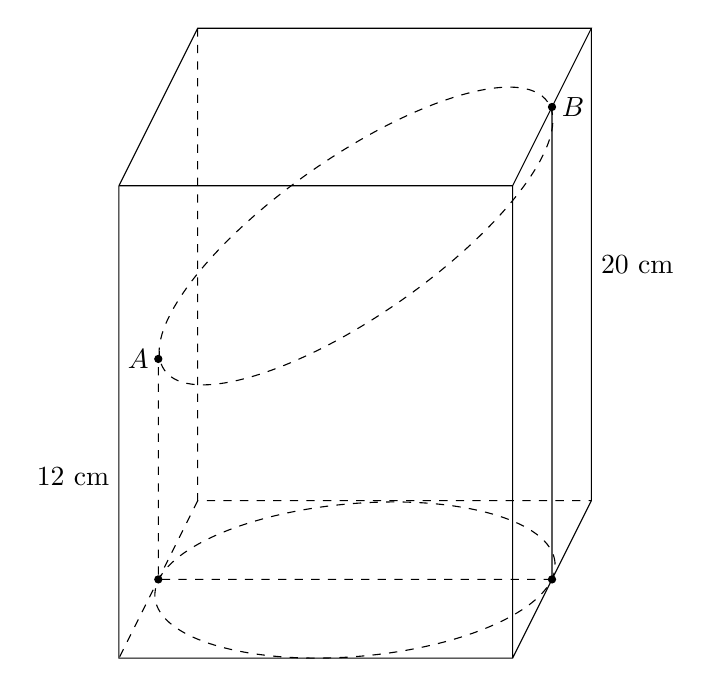
\begin{tikzpicture}
			\draw (0,0) -- (5,0) -- (6,2) -- (1,2) -- (0,0);
			\draw (0,0) -- (0,-6) -- (5,-6) -- (5,0) (5,-6) -- (6,-4) -- (6,2) (5.5,-5) -- (5.5,1);
			\draw[dashed] (1,2) -- (1,-4) -- (6,-4) (1,-4) -- (0,-6) (5.5,-5) -- (0.5,-5) -- (0.5,-2.2);
			\draw[dashed,rotate=5,shift={(-0.45 cm,-0.25 cm)}] (3,-5) ellipse (2.55cm and 0.97cm);
			\draw[dashed,rotate=35,shift={(-0.9 cm,-0.25 cm)}] (3,-2) ellipse (2.97cm and 1cm);
			\fill (0.5,-2.2) circle (1.5pt);
			\fill (5.5,1) circle (1.5pt);
			\fill (0.5,-5) circle (1.5pt);
			\fill (5.5,-5) circle (1.5pt);
			\node[left] at (0,-3.7) {$12$ cm};
			\node[right] at (6,-1) {$20$ cm};
			\node[left] at (0.5,-2.2) {$A$};
			\node[right] at (5.5,1) {$B$};
		\end{tikzpicture}
	\end{center}
	\choice
	{$R=5,2$ cm}
	{$R=4,8$ cm}
	{$R=6,4$ cm}
	{\True $R=8,2$ cm}
	\loigiai{
		\begin{center}
			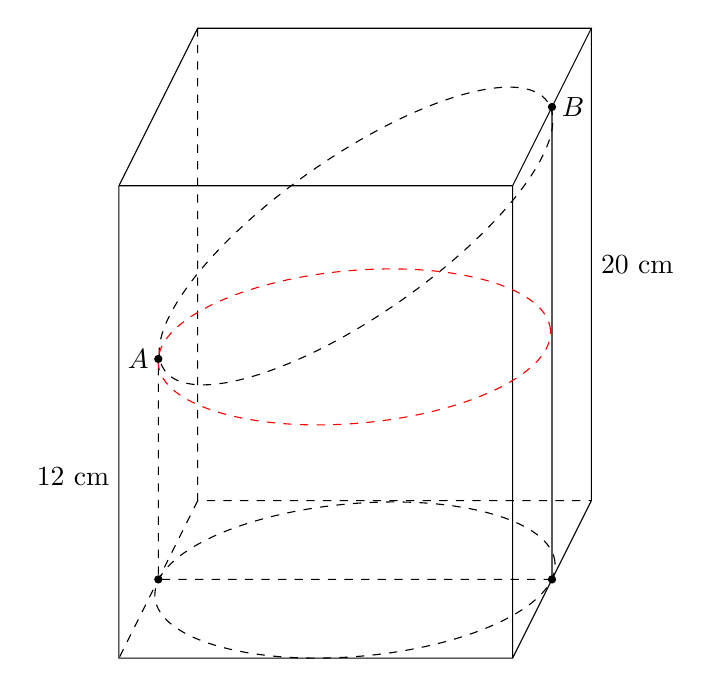
\begin{tikzpicture}
				\draw (0,0) -- (5,0) -- (6,2) -- (1,2) -- (0,0);
				\draw (0,0) -- (0,-6) -- (5,-6) -- (5,0) (5,-6) -- (6,-4) -- (6,2) (5.5,-5) -- (5.5,1);
				\draw[dashed] (1,2) -- (1,-4) -- (6,-4) (1,-4) -- (0,-6) (5.5,-5) -- (0.5,-5) -- (0.5,-2.2);
				\draw[dashed,rotate=5,shift={(-0.45 cm,-0.25 cm)}] (3,-5) ellipse (2.55cm and 0.97cm);
				\draw[dashed,rotate=35,shift={(-0.9 cm,-0.25 cm)}] (3,-2) ellipse (2.97cm and 1cm);
				\draw[red,dashed,rotate=5,shift={(-0.2 cm,2.7 cm)}] (3,-5) ellipse (2.5cm and 0.97cm);
				\fill (0.5,-2.2) circle (1.5pt);
				\fill (5.5,1) circle (1.5pt);
				\fill (0.5,-5) circle (1.5pt);
				\fill (5.5,-5) circle (1.5pt);
				\node[left] at (0,-3.7) {$12$ cm};
				\node[right] at (6,-1) {$20$ cm};
				\node[left] at (0.5,-2.2) {$A$};
				\node[right] at (5.5,1) {$B$};
			\end{tikzpicture}
		\end{center}
		Gọi bán kính đáy hình trụ là $R$.\\
		Gọi $V_1,V_2$ lần lượt là thể tích hình hộp chữ nhật và khối gỗ.\\
		Ta có $V_1=B\cdot h=4R^2\cdot 20=80R^2$.\\
		Chia khối gỗ làm hai phần bằng một mặt phẳng qua $A$ và song song đáy.\\
		Ta có $V_2=\pi{R^2}\cdot h_1+\dfrac{1}{2}\pi{R^2}\cdot \left(h-h_1\right)=16\pi{R^2}.$\\
		$h_1$ là khoảng cách từ điểm $A$ đến mặt đáy, $h$ khoảng cách từ điểm $B$ đến mặt đáy.\\
		Thể tích nước còn lại là\\
		$V=V_1-V_2=16R^2\left(5-\pi\right)=2000\Rightarrow R\approx 8,2$.}
\end{ex}

\begin{ex}%Câu 17 [2H2B1-4]	[Ngô Quyền-Hải Phòng 2019] 
	Một hộp đựng bóng tennis có dạng hình trụ. Biết rằng hộp chứa vừa khít ba quả bóng tennis được xếp theo chiều dọc, các quả bóng tennis có kích thước như nhau. Thể tích phần không gian còn trống chiếm tỉ lệ $a\%$ so với hộp đựng bóng tennis. Số $a$ gần đúng với số nào sau đây?
	\choice
	{$50$}
	{$66$}
	{$30$}
	{\True $33$}
	\loigiai{
		\begin{center}
			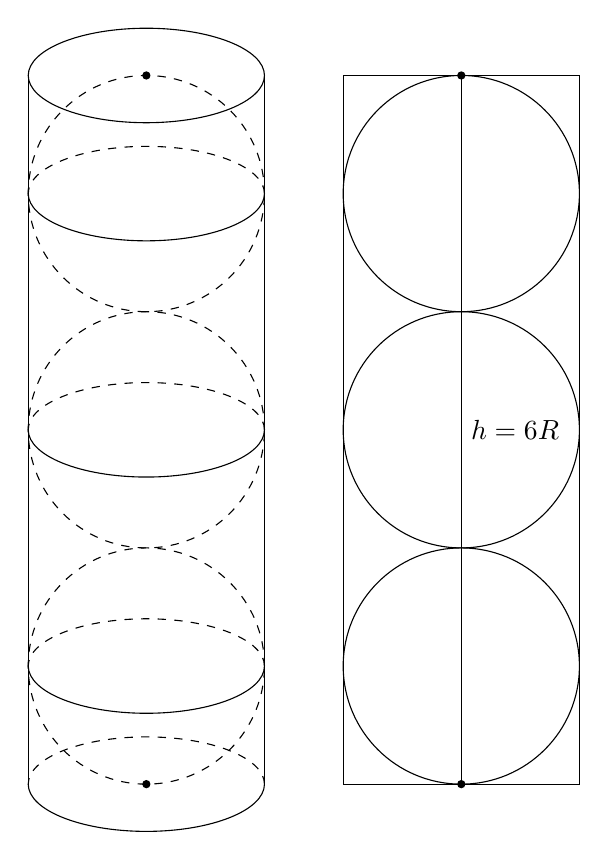
\begin{tikzpicture}
				\draw (0,0) ellipse (1.5cm and 0.6cm);
				\draw (-1.5,0) -- (-1.5,-9);
				\draw (1.5,0) -- (1.5,-9);
				\draw (-1.5,-7.5) arc (180:360:1.5cm and 0.6cm);
				\draw[dashed] (1.5,-1.5) arc (0:180:1.5cm and 0.6cm);
				\draw (-1.5,-4.5) arc (180:360:1.5cm and 0.6cm);
				\draw[dashed] (1.5,-4.5) arc (0:180:1.5cm and 0.6cm);
				\draw (-1.5,-1.5) arc (180:360:1.5cm and 0.6cm);
				\draw[dashed] (1.5,-7.5) arc (0:180:1.5cm and 0.6cm);
				\draw (-1.5,-9) arc (180:360:1.5cm and 0.6cm);
				\draw[dashed] (0,-1.5) circle (1.5cm);
				\draw[dashed] (0,-4.5) circle (1.5cm);
				\draw[dashed] (0,-7.5) circle (1.5cm);
				\fill (0,0) circle (1.5pt);
				\fill (0,-9) circle (1.5pt);
				\draw[dashed] (1.5,-9) arc (0:180:1.5cm and 0.6cm);
				\draw (4,-1.5) circle (1.5cm);
				\draw (4,-4.5) circle (1.5cm);
				\draw (4,-7.5) circle (1.5cm);
				\draw (5.5,0) rectangle (2.5,-9);
				\draw (4,0) -- (4,-9);
				\fill (4,0) circle (1.5pt);
				\fill (4,-9) circle (1.5pt);
				\node[right] at (4,-4.5) {$h=6R$};
			\end{tikzpicture}
		\end{center}
		Đặt $h,R$ lần lượt là đường cao và bán kính hình tròn đáy của hộp đựng bóng tennis.\\
		Dễ thấy mỗi quả bóng tennis có cùng bán kính $R$ với hình tròn đáy của hộp đựng bóng tennis và $h=6R$.\\
		Tổng thể tích của ba quả bóng là $V_1=3\cdot \dfrac{4}{3}\pi{R^3}=4\pi{R^3}$.\\
		Thể tích của hình trụ (hộp đựng bóng) là $V_0=\pi{R^2}h=6\pi{R^3}$.\\
		Thể tích phần còn trống của hộp đựng bóng là $V_2=V_0-V_1=2\pi{R^3}$.\\
		Khi đó tỉ lệ phần không gian còn trống so với hộp đựng bóng là $\dfrac{V_2}{V_0}=\dfrac{1}{3}\approx 0,33$.\\
		Suy ra $a\approx 33$.}
\end{ex}
%%%%---18-25
\begin{ex}%[2H2T1-5][Chuyên Ngữ Hà Nội 2019]
	Sử dụng mảnh inox hình chữ nhật $ABCD$ có diện tích bằng $1\, \mathrm{m}^2$ và cạnh $BC=x\, (\mathrm{m})$ để làm một thùng đựng nước có đáy, không có nắp theo quy trình như sau: Chia hình chữ nhật $ABCD$ thành hai hình chữ nhật $ADNM$ và $BCNM$, trong đó phần hình chữ nhật $ADNM$ được gò thành phần xung quanh hình trụ có chiều cao bằng $AM$; phần hình chữ nhật $BCNM$ được cắt ra một hình tròn để làm đáy của hình trụ trên (phần inox còn thừa được bỏ đi). Tính gần đúng giá trị $x$ để thùng nước trên có thể tích lớn nhất (coi như các mép nối không đáng kể).
	\begin{center}
		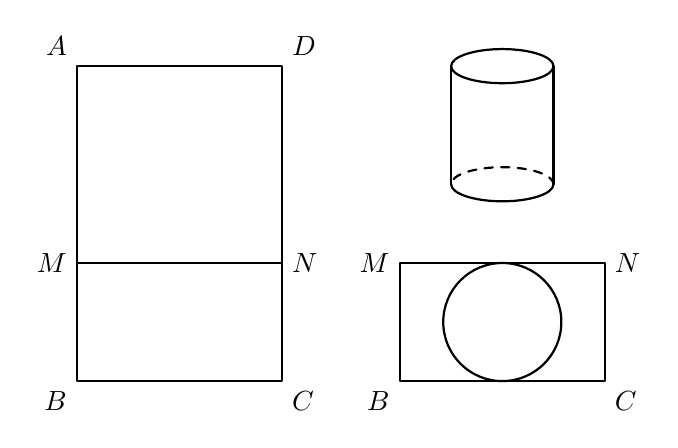
\begin{tikzpicture}[line join = round, line cap = round, scale = 1, thick]
			\pgfmathsetmacro\bchalf{1.3}
			\pgfmathsetmacro\r{\bchalf/2}
			\pgfmathsetmacro\ab{4}
			\pgfmathsetmacro\bm{1.5}
			\pgfmathsetmacro\h{\ab-\bm-1}
			\tikzset{abcd/.pic={
					\draw (-\bchalf,0) node[below left]{$B$} rectangle (\bchalf,\ab) node[above right]{$D$};
					\draw (-\bchalf,\bm) node[left]{$M$}--(\bchalf,\bm) node[right]{$N$};
					\path (-\bchalf,\ab) node[above left]{$A$} (\bchalf,0) node[below right]{$C$};
			}}
			\tikzset{bcnm/.pic={
					\draw (-\bchalf,0) node[below left]{$B$}--++(0,\bm) node[left]{$M$}--++({2*\bchalf},0) node[right]{$N$} --++(0,-\bm) node[below right]{$C$}--cycle;
					\draw (0,{\bm/2}) circle (\bm/2);
			}}
			\tikzset{tru/.pic={
					\draw[dashed] (\r,0) arc(0:180:{\r} and {\r/3});
					\draw (\r,\h) arc(0:180:{\r} and \r/3);
					\draw (-\r,0) arc(180:360:{\r} and \r/3);
					\draw (-\r,\h) arc(180:360:{\r} and \r/3);
					\draw (-\r,0)--(-\r,\h) (\r,0)--(\r,\h);
			}}
			\draw (0,0) pic{abcd} (2*\bchalf+1.5,0) pic{bcnm} ({2*\bchalf+1.5},{\bm+1}) pic{tru};
		\end{tikzpicture}
	\end{center}
	\choice
	{$1{,}37\, \mathrm{m}$}
	{\True $1{,}02\, \mathrm{m}$}
	{$0{,}97\,\mathrm{m}$}
	{$1\,\mathrm{m}$}
	\loigiai
	{
		Ta có $AB\cdot BC=1\Rightarrow AB=\dfrac{1}{BC}=\dfrac{1}{x}$.\\
		Gọi $R$ là bán kính đáy hình trụ inox gò được, ta có chu vi hình tròn đáy bằng $BC=x$.\\
		Do đó $2\pi R=x \Leftrightarrow R=\dfrac{x}{2\pi}$; $BM=2R=\dfrac{x}{\pi}\Rightarrow AM=AB-BM=\dfrac{1}{x}-\dfrac{x}{\pi}$.\\
		Thể tích khối trụ inox gò được là $V=\pi{R^2}h=\pi \left(\dfrac{x}{2\pi}\right)^2\left(\dfrac{1}{x}-\dfrac{x}{\pi}\right)=\dfrac{1}{4\pi^2}x\left(\pi-x^2\right)$.\\
		Xét hàm số $f(x)=x\left(\pi-x^2\right), x>0$. Ta có $f'(x)=\pi-3x^2$, $f'(x)=0 \Leftrightarrow \hoac{&x=\sqrt{\dfrac{\pi}{3}}\\ &x=-\sqrt{\dfrac{\pi}{3}}\; \text{(loại)}} $.\\
		%$f'(x)=0$ $\Rightarrow $ $x=\sqrt{\dfrac{\pi}{3}}$ ; $f'(x)>0$ $\Leftrightarrow $ $x\in\left(0;\sqrt{\dfrac{\pi}{3}}\right)$ và $f'(x)<0$ $\Leftrightarrow $ $x\in\left(\sqrt{\dfrac{\pi}{3}};+\infty\right)$ .\\
		%Vậy $f(x)$ đồng biến trên khoảng $\left(0;\sqrt{\dfrac{\pi}{3}}\right)$ và nghịch biến trên khoảng $\left(\sqrt{\dfrac{\pi}{3}};+\infty\right)$ .\\
		Ta có bảng biến thiên
		\begin{center}
			
\begin{tikzpicture}[double distance = 3pt]
				\tkzTabInit[lgt=1.5,espcl=2.5, nocadre]{$x$/1.2, $f'(x)$/.7, $f(x)$/2}{$0$, $\sqrt{\dfrac{\pi}{3}}$, $+\infty$}
				\tkzTabLine{,+,0,-,}
				\tkzTabVar{-/,+/$\dfrac{2\pi\sqrt{3\pi}}{9}$,-/}
			\end{tikzpicture}
		\end{center}
		Từ bảng biến thiên ta suy ra $\underset{\left(0;+\infty\right)}{\max}\,f(x)=f\left(\sqrt{\dfrac{\pi}{3}}\right)=\dfrac{2\pi\sqrt{3\pi}}{9}$.\\
		Từ đó ta có thể tích $V$ lớn nhất khi và chỉ khi $f(x)$ lớn nhất, khi đó  $x=\sqrt{\dfrac{\pi}{3}}\approx 1{,}02$ $(\mathrm{m})$.}
\end{ex}

\begin{ex}%[2H2T1-5]
	Một đại lý xăng dầu cần làm một cái bồn dầu hình trụ bằng tôn có thể tích $16\pi\, (\mathrm{m}^3)$. Tìm bán kính đáy $r$ của hình trụ sao cho hình trụ được làm ra ít tốn nguyên vật liệu nhất.
	\choice
	{$0{,}8\, \mathrm{m}$}
	{$1{,}2\, \mathrm{m}$}
	{\True $2\, \mathrm{m}$}
	{$2{,}4\, \mathrm{m}$}
	\loigiai
	{Để ít tốn nguyên vật liệu nhất thì diện tích toàn phần $S_{\text{tp}}$ phải nhỏ nhất.\\
		Gọi $h$ $\left(h>0\right)$ là chiều cao của bồn dầu. Ta có $S_{\text{tp}}=2\pi{r^2}+2\pi rh$.\\
		Mặt khác, theo giả thiết $V=16\pi\Leftrightarrow\pi{r^2}h=16\pi\Leftrightarrow h=\dfrac{16}{r^2}$.\\
		Khi đó ${S_{\text{tp}}}=2\pi{r^2}+2\pi r\cdot\dfrac{16}{r^2}=2\pi\left(r^2+\dfrac{16}{r}\right)=2\pi\left(r^2+\dfrac{8}{r}+\dfrac{8}{r}\right)$.\\
		Áp dụng BĐT Cauchy cho 3 số dương $r^2, \dfrac{8}{r}, \dfrac{8}{r}$ ta được $r^2+\dfrac{8}{r}+\dfrac{8}{r}\ge 3\sqrt[3]{r^2\cdot\dfrac{8}{r}\cdot\dfrac{8}{r}}=12$.\\
		Do đó ${S_{\text{tp}}}\ge 24\pi $. Đẳng thức xảy ra $\Leftrightarrow{r^2}=\dfrac{8}{r}\Leftrightarrow{r^3}=8\Leftrightarrow r=2$ .\\
		Vậy để ít tốn nguyên vật liệu nhất thì $r=2\, (\mathrm{m})$.}
\end{ex}

\begin{ex}%[2H2T1-5][THPT Cẩm Bình Hà Tỉnh 2019]
	Anh H dự định làm một cái thùng đựng dầu hình trụ bằng sắt có nắp đậy thể tích $12\,\mathrm{m}^3$. Chi phí làm mỗi $\mathrm{m}^2$ đáy là $400$ ngàn đồng, mỗi $\mathrm{m}^2$ nắp là $200$ ngàn đồng, mỗi $\mathrm{m}^2$ mặt xung quanh là $300$ ngàn đồng. Để chi phí làm thùng là ít nhất thì anh H cần chọn chiều cao của thùng gần nhất với số nào sau đây? (Xem độ dày của tấm sắt làm thùng là không đáng kể).
	\choice
	{$1{,}24\,\mathrm{m}$}
	{$1{,}25\,\mathrm{m}$}
	{$2{,}50\,\mathrm{m}$}
	{\True $2{,}48\,\mathrm{m}$}
	\loigiai
	{Gọi bán kính đáy của hình trụ là $R$. Ta có $V=\pi{R^2}h\Rightarrow h=\dfrac{12}{\pi{R^2}}$.\\
		Suy ra chi phí (đơn vị ngàn đồng) làm thùng\\
		\begin{align*}
			C&=\pi{R^2}\cdot 400+\pi{R^2}\cdot 200+2\pi Rh\cdot 300\\
			&=600\left(\pi{R^2}+\dfrac{12}{R}\right)=600\left(\pi{R^2}+\dfrac{6}{R}+\dfrac{6}{R}\right)\\
			&\ge 600.3\sqrt[3]{\pi{R^2}.\dfrac{6}{R}.\dfrac{6}{R}}=1800\sqrt[3]{36\pi}.
		\end{align*}
		Dẫn dến giá trị nhỏ nhất của $C$ là $1800\sqrt[3]{36\pi}$, đạt được khi và chỉ khi ${R^2}=\dfrac{6}{R}\Leftrightarrow R=\sqrt[3]{\dfrac{6}{\pi}}$.\\
		Vậy để chi phí nhỏ nhất thì chiều cao của hình trụ là $h=\dfrac{12}{\sqrt[3]{36\pi}}\approx 2{,}48\,\mathrm{m}$.}
\end{ex}

\begin{ex}%[2H2T1-5][Bỉm Sơn - Thanh Hóa - 2019]
	Người ta cần làm một cái bồn chứa dạng hình trụ có thể tích $1000$ lít bằng inox để chứa nước, tính bán kính $R$ của hình trụ đó sao cho diện tích toàn phần của bồn chứa có giá trị nhỏ nhất.
	\choice
	{$R=\sqrt[3]{\dfrac{2}{\pi}}$}
	{$R=\sqrt[3]{\dfrac{1}{\pi}}$}
	{\True $R=\sqrt[3]{\dfrac{1}{2\pi}}$}
	{$R=\sqrt[3]{\dfrac{3}{2\pi}}$}
	\loigiai
	{Ta có $1000\; \text{lít} = 1\, \mathrm{m}^3$.\\
		Gọi $h$ là chiều cao của hình trụ ta có $V=\pi{R^2}h=1\Rightarrow h=\dfrac{1}{\pi{R^2}}$.\\
		Diện tích toàn phần là 
		\begin{align*}
			S_{\mathrm{tp}}&=2\pi{R^2}+2\pi Rh=2\pi{R^2}+2\pi R\cdot \dfrac{1}{\pi{R^2}}=2\pi{R^2}+\dfrac{2}{R}\\
			&=2\left(\pi{R^2}+\dfrac{1}{2R}+\dfrac{1}{2R}\right)\ge 2.3\sqrt[3]{\pi{R^2}.\dfrac{1}{2R}.\dfrac{1}{2R}}=6\sqrt[3]{\dfrac{\pi}{4}}
		\end{align*}
		Dấu bằng xảy ra khi và chỉ khi $\pi{R^2}=\dfrac{1}{2R}\Leftrightarrow R=\sqrt[3]{\dfrac{1}{2\pi}}$.}
\end{ex}

\begin{ex}%[2H2K1-5][Chuyên Vĩnh Phúc - 2020]
	Thiết diện của hình trụ và mặt phẳng chứa trục của hình trụ là hình chữ nhật có chu vi bằng $12$. Giá trị lớn nhất của thể tích khối trụ là
	\choice
	{$16\pi $}
	{$32\pi $}
	{\True $8\pi $}
	{$64\pi $}
	\loigiai
	{
		\begin{center}
			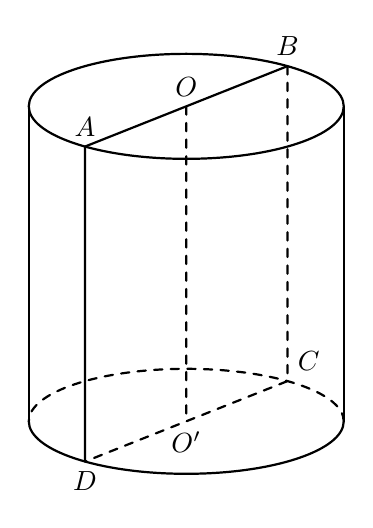
\begin{tikzpicture}[line join = round, line cap = round, scale = 1, thick]
				\def\h{4}
				\def\angle{50}
				\pgfmathsetmacro{\r}{2}
				\draw (0,0) coordinate (J) node[below]{$O'$}
				(0,\h) coordinate (I) node[above]{$O$};
				\draw (I) ellipse ({\r} and {\r/3});
				\draw (-\r,0) arc (180:360: {\r}  and {\r/3} );
				\draw[dashed] (\r,0) arc(0:180: {\r}  and {\r/3} );
				\draw (-\r,0)--(-\r,\h) (\r,0)--(\r,\h);
				\draw (I)++(\angle:{\r} and {\r/3}) coordinate (B) node[above]{$B$} (I)++(180+\angle:{\r} and {\r/3}) coordinate (A) node[above]{$A$};
				\draw (J)++(\angle:{\r} and {\r/3}) coordinate (C) node[above right]{$C$} (J)++(180+\angle:{\r} and {\r/3}) coordinate (D) node[below]{$D$};
				\draw (B)--(A)--(D);
				\draw[dashed] (B)--(C)--(D) (I)--(J);
			\end{tikzpicture}
		\end{center}
		Từ hình vẽ ta có $ABCD$ là hình chữ nhật, gọi chiều cao của hình trụ là $h$ và bán kính đáy của hình trụ là $r$, theo giả thiết ta có $2(h+2r)=12\Leftrightarrow h+2r=6$.\\
		Thể tích của khối trụ tương ứng là $V=\pi{r^2}h$.\\
		Theo bất đẳng thức Cauchy ta có $r+r+h\ge 3\sqrt[3]{r^2.h}\Rightarrow V=\pi{r^2}h\le\pi \cdot \left(\dfrac{2r+h}{3}\right)^3=8\pi$.\\
		Dấu bằng xảy ra khi và chỉ khi $r=h=2$.\\
		Vậy giá trị lớn nhất của thể tích khối trụ là $8\pi $.}
\end{ex}

\begin{ex}%[2H2T1-5][Chuyên Nguyễn Trãi Hải Dương 2019]
	Cần sản xuất một vỏ hộp sữa hình trụ có thể tích $V$ cho trước. Để tiết kiệm vật liệu nhất thì bán kính đáy phải bằng
	\choice
	{\True $\sqrt[3]{\dfrac{V}{2\pi}}$}
	{$\sqrt[3]{\dfrac{V}{2}}$}
	{$\sqrt[3]{\dfrac{V}{\pi}}$}
	{$\sqrt[3]{\dfrac{V}{3\pi}}$}
	\loigiai
	{Gọi $h, r$ là chiều cao và bán kính đường tròn đáy của hình trụ. Ta có $V=\pi{r^2}h\Leftrightarrow h=\dfrac{V}{\pi{r^2}}$.\\
		Để tiết kiệm vật liệu nhất thì diện tích toàn phần nhỏ nhất.\\
		Ta có $S_{\mathrm{tp}}=2\pi{r^2}+2\pi rh=2\pi{r^2}+2\pi r\dfrac{V}{\pi{r^2}}=2\pi{r^2}+\dfrac{2V}{r}=2\pi{r^2}+\dfrac{V}{r}+\dfrac{V}{r}$.\\
		Áp dụng BĐT AM - GM cho ba số $2\pi{r^2}, \dfrac{V}{r},\dfrac{V}{r}$ ta có $S_{tp}\ge 3\sqrt[3]{2\pi{r^2}\cdot \dfrac{V}{r}\cdot \dfrac{V}{r}}=3\sqrt[3]{\dfrac{2\pi{V^2}}{r}}$ không đổi.\\
		Dấu bằng xảy ra khi và chỉ khi $2\pi{r^2}=\,\dfrac{V}{r}\Leftrightarrow r=\sqrt[3]{\dfrac{V}{2\pi}}$.}
\end{ex}

\begin{ex}%[2H2K1-5][ĐHQG Hà Nội - 2020]
	Trong các hình trụ có diện tích toàn phần bằng $1000\,{\mathrm{cm}^2}$ thì hình trụ có thể tích lớn nhất là bao nhiêu $\mathrm{cm}^3$?
	\choice
	{\True $2428$}
	{$2532$}
	{$2612$}
	{$2740$}
	\loigiai{
		Đặt $S=1000$ là diện tích toàn phần của hình trụ. Ta có $S=2\pi Rh+2\pi{R^2}\Rightarrow Rh+R^2=\dfrac{S}{2\pi}$.\\
		Vậy thể tích khối trụ là $V=\pi{R^2}h=\pi R\left(\dfrac{S}{2\pi}-R^2\right)=\dfrac{S}{2}R-\pi{R^3}$.\\
		Xét hàm số $f(R)=\dfrac{S}{2}R-\pi{R^3}, R>0$. Ta có $f'(R)=\dfrac{S}{2}-3\pi{R^2}=0\Leftrightarrow \hoac{&R=\sqrt{\dfrac{S}{6\pi}}\\&R=-\sqrt{\dfrac{S}{6\pi}}\;\text{(loại)}}$.\\
		Bảng biến thiên:
		\begin{center}
			
\begin{tikzpicture}[double distance = 3pt]
				\tkzTabInit[lgt=1.5,espcl=2.5, nocadre]{$R$/1.3, $f'(R)$/.7, $f(R)$/2.5}{$0$, $\sqrt{\dfrac{S}{6\pi}}$, $+\infty$}
				\tkzTabLine{,+,0,-,}
				\tkzTabVar{-/, +/$f\left(\sqrt{\dfrac{S}{6\pi}}\right)$,-/}
			\end{tikzpicture}
		\end{center}
		Từ bảng biến thiên ta có $V_{\max}=\dfrac{S}{2}R-\pi{R^3}=\dfrac{1000}{2}\sqrt{\dfrac{1000}{6\pi}}-\pi{\sqrt{\dfrac{1000}{6\pi}}^3}\approx 2428.$}
\end{ex}

\begin{ex}%[2H2G1-5][Tiên Lãng - Hải Phòng - 2020]
	Cho hình trụ có đáy là hai đường tròn tâm $O$ và $O'$, bán kính đáy bằng chiều cao và bằng $2a$. Trên đường tròn đáy có tâm $O$ lấy điểm $A$, trên đường tròn tâm $O'$ lấy điểm $B$. Đặt $\alpha $ là góc giữa $AB$ và đáy. Biết rằng thể tích khối tứ diện $O{O}'AB$ đạt giá trị lớn nhất. Khẳng định nào sau đây đúng?
	\choice
	{$\tan\alpha=\sqrt{2}$}
	{$\tan\alpha=1$}
	{\True $\tan\alpha=\dfrac{1}{\sqrt{2}}$}
	{$\tan\alpha=\dfrac{1}{2}$}
	\loigiai
	{
		\begin{center}
			\begin{tikzpicture}[line join = round, line cap = round, scale = 1, thick]
				\def\h{4}
				\pgfmathsetmacro{\r}{2}
				\draw (0,0) coordinate (J) node[right]{$O$}
				(0,\h) coordinate (I) node[right]{$O'$};
				\draw (I) ellipse ({\r} and {\r/3});
				\draw (-\r,0) arc (180:360: {\r}  and {\r/3} );
				\draw[dashed] (\r,0) arc(0:180: {\r}  and {\r/3} );
				\draw (-\r,0)--(-\r,\h) (\r,0)--(\r,\h);
				\draw (I)++(110:{\r} and {\r/3}) coordinate (B) node[above left]{$B$};
				\draw (J)++(110:{\r} and {\r/3}) coordinate (B') node[above left]{$B'$};
				\draw (J)++(-150:{\r} and {\r/3}) coordinate (A) node[below]{$A$};
				\draw ($(A)!.5!(B')$) coordinate (H) node[above]{$H$};
				\draw[dashed] (A)--(B)--(B')--(A) (J)--(H);
				\draw[dashed] (I)--(J)--(B');
				\draw[dashed] (J)--(A)--(I) (B)--(J);
				\draw (B)--(I);
			\end{tikzpicture}
		\end{center}
		Gọi $B'$ là hình chiếu của $B$ trên mặt phẳng chứa đường tròn $(O)$ , khi đó $A{B}'$ là hình chiếu của $AB$ trên mặt phẳng chứa đường tròn $(O)$ .\\
		Suy ra $\left(\widehat{AB,\left(OA{B}'\right)}\right)=\left(\widehat{AB,A{B}'}\right)=\widehat{BA{B}'}=\alpha $ , $\alpha\in\left(0;\dfrac{\pi}{2}\right)$ .\\
		Xét tam giác vuông $AB{B}'$ vuông tại $B'$ có $\tan\widehat{BA{B}'}=\dfrac{B{B}'}{A{B}'}$ $\Rightarrow A{B}'=\dfrac{B{B}'}{\tan\alpha}=\dfrac{2a}{\tan\alpha}$ .\\
		Gọi $H$ là trung điểm $A{B}'$ , khi đó $OH\perp A{B}'$ và
		$$OH=\sqrt{O{A^2}-A{H^2}}=\sqrt{R^2-\dfrac{A{B'^2}}{4}}=\sqrt{4a^2-\dfrac{a^2}{\tan^2\alpha}}=a\sqrt{4-\dfrac{1}{\tan^2\alpha}}.$$
		Lại có $S_{\triangle OA{B}'}=\dfrac{1}{2}OH.A{B}'=\dfrac{1}{2}.O{B}'. \mathrm{d} \left(A,O{B}'\right)$. Suy ra
		$$ d\left(A,O{B}'\right)=\dfrac{OH.A{B}'}{O{B}'}=\dfrac{a\sqrt{4-\dfrac{1}{\tan^2\alpha}}\cdot \dfrac{2a}{\tan\alpha}}{2a}=\dfrac{a}{\tan\alpha}\sqrt{4-\dfrac{1}{\tan^2\alpha}}=\mathrm{d}\left(A,\left(O{O}'B{B}'\right)\right).$$
		Vậy nên
		\begin{align*}
			V_{A.O{O}'B}&=\dfrac{1}{3}\mathrm{d}\left(A,\left(O{O}'B{B}'\right)\right).S_{\triangle OO'B}\\
			&=\dfrac{1}{3}\cdot \dfrac{a}{\tan\alpha}\sqrt{4-\dfrac{1}{\tan^2\alpha}}\cdot \dfrac{1}{2}\cdot 2a\cdot 2a=\dfrac{2a^3}{3}\cdot \dfrac{1}{\tan\alpha}\sqrt{4-\dfrac{1}{\tan^2\alpha}}.
		\end{align*}
		Áp dụng bất đẳng thức Cauchy ta có $$\dfrac{1}{\tan\alpha}\sqrt{4-\dfrac{1}{\tan^2\alpha}}\le\dfrac{\dfrac{1}{\tan^2\alpha}+4-\dfrac{1}{\tan^2\alpha}}{2}=2.$$
		Do đó ${V_{A.O{O}'B}}\le\dfrac{2a^3}{3}\cdot 2=\dfrac{4a^3}{3}.$\\
		Dấu bằng xảy ra khi và chỉ khi $\dfrac{1}{\tan\alpha}=\sqrt{4-\dfrac{1}{\tan^2\alpha}}\Leftrightarrow\dfrac{1}{\tan^2\alpha}=4-\dfrac{1}{\tan^2\alpha}\Leftrightarrow{\tan^2}\alpha=\dfrac{1}{2}$.\\
		Vì $\alpha\in \left(0;\dfrac{\pi}{2}\right)$ nên $\tan\alpha=\dfrac{1}{\sqrt{2}}$ do $\alpha\in\left(0;\dfrac{\pi}{2}\right)$.}
\end{ex}
%%%%---26-33
\begin{ex}%Câu 26 [2H2G1-5]
	Cho hình trụ có đáy là hai đường tròn tâm $O$ và $O'$, bán kính đáy bằng chiều cao và bằng $2a$. Trên đường tròn đáy có tâm $O$ lấy điểm $A$, trên đường tròn tâm $O'$ lấy điểm $B$. Đặt $\alpha $ là góc giữa $AB$ và đáy. Tính $\tan\alpha $ khi thể tích khối tứ diện $O{O}'AB$ đạt giá trị lớn nhất.
	\choice
	{$\tan\alpha=\dfrac{1}{2}$}
	{\True$\tan\alpha=\dfrac{1}{\sqrt{2}}$}
	{$\tan\alpha=1$}
	{$\tan\alpha=\sqrt{2}$}
	\loigiai
	{	\begin{center}
			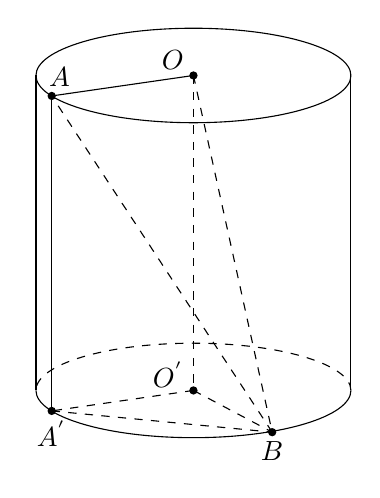
\begin{tikzpicture}[scale=1]
				\draw (0,0) ellipse (2cm and 0.6cm);
				\draw (-2,0) -- (-2,-4);
				\draw (2,0) -- (2,-4);
				\draw (-2,-4) arc (180:360:2cm and 0.6cm);
				\draw[dashed] (2,-4) arc (0:180:2cm and 0.6cm);
				\node[left] at (0,0.2) {\normalsize$O$};
				\fill (0,0) circle (1.5pt);
				\node[left] at (0,-3.8) {\normalsize$O^{'}$};
				\draw[dashed] (0,0) -- (0,-4);
				\fill (0,-4) circle (1.5pt);
				\fill (-1.8,-0.26) circle (1.5pt);
				\node[above] at (-1.7,-0.26) {\normalsize$A$};
				\fill (1,-4.53) circle (1.5pt);
				\node[below] at (1,-4.53) {\normalsize$B$};
				\fill (-1.8,-4.26) circle (1.5pt);
				\node[below] at (-1.8,-4.26) {\normalsize$A^{'}$};
				\draw (0,0) -- (-1.8,-0.26);
				\draw (-1.8,-4.26) -- (-1.8,-0.26);
				\draw[dashed] (-1.8,-4.26) -- (1,-4.53);
				\draw[dashed] (0,0) -- (1,-4.53);
				\draw[dashed] (0,-4) -- (1,-4.53);
				\draw[dashed] (0,-4) -- (-1.8,-4.26);
				\draw[dashed] (1,-4.53) -- (-1.8,-0.26);
			\end{tikzpicture}
		\end{center}
		Gọi $A'$ là hình chiếu của $A$ trên đường tròn tâm $O'$ khi đó ta có\\ $V_{OO'AB}=\dfrac{1}{2}{V_{B.OO'A'A}}=\dfrac{1}{6}\cdot S_{OO'A'A}\cdot \mathrm{\,d}\left(B,\left(OO'A'A\right)\right)$ với $\mathrm{\,d}\left(B,\left(OO'A'A\right)\right)=OB\cdot\sin\widehat{BO'A'}$.\\
		Do $S_{OO'A'A}$ là hằng số nên để thể tích khối tứ diện $O{O}'AB$ đạt giá trị lớn nhất thì $\mathrm{\,d}\left(B,\left(OO'A'A\right)\right)$ là lớn nhất hay $\widehat{BO'A'}=90^0$.\\
		Khi đó ta có $\tan\alpha=\tan\widehat{ABA'}=\dfrac{AA'}{A'B}=\dfrac{2a}{2a\sqrt{2}}=\dfrac{\sqrt{2}}{2}$.}
\end{ex}
\begin{ex}%Câu 27 [2H2G1-4]
	Một xí nghiệp chế biến sữa bò muốn sản xuất lon đựng sữa có dạng hình trụ bằng thiếc có thể tích không đổi. Để giảm giá một lon sữa khi bán ra thị trường người ta cần chế tạo lon sữa có kích thước sao cho ít tốn kém vật liệu. Để thỏa mãn yêu cầu đặt ra (diện tích toàn phần bé nhất), người ta phải thiết kế lon sữa thỏa mãn điều kiện nào trong các điều kiện sau:
	\choice
	{\True Chiều cao bằng đường kính của đáy}
	{Chiều cao bằng bán kính của đáy}
	{Chiều cao bằng 3 lần bán kính của đáy}
	{Chiều cao bằng bình phương bán kính của đáy}
	\loigiai
	{
		Gọi $V$ , $r$ , $h$ , $\ell$ lần lượt là thể tích, bán kính đáy, đường cao, đường sinh của lon sữa.\\
		Ta có: $V=\pi .r^2.h\Rightarrow h=\dfrac{V}{\pi .r^2}$ và $h=\ell$.\\
		Mặt khác: $V=\pi .r^2.h\Rightarrow h=\dfrac{V}{\pi .r^2}$.\\
		$S_{tp}=2\pi r\ell+2\pi{r^2}=2\pi r\cdot\dfrac{V}{\pi .r^2}+2\pi{r^2}=\dfrac{2V}{r}+2\pi{r^2}=\dfrac{V}{r}+\dfrac{V}{r}+2\pi{r^2}$ .\\
		Áp dụng bất đẳng thức Côsi cho 3 số dương ta được:\\
		$S_{tp}\ge 3\sqrt[3]{\dfrac{V}{r}\cdot\dfrac{V}{r}\cdot 2\pi{r^2}}=3\sqrt[3]{2\pi{V^2}}$ .\\
		Đẳng thức xảy ra khi $\dfrac{V}{r}=2\pi{r^2}\Leftrightarrow\dfrac{V}{\pi}=2r^3$ . Do $h=\dfrac{V}{\pi .r^2}$ nên $2r=h$.}
\end{ex}
\begin{ex}%Câu 28 [2H2G1-5]
	Người ta thiết kế một thùng chứa hình trụ (như hình vẽ) có thể tích $V$ nhất định. Biết rằng giá của vật liệu làm mặt đáy và nắp của thùng bằng nhau và đắt gấp ba lần so với giá vật liệu để làm mặt xung quanh của thùng (chi phí cho mỗi đơn vị diện tích). Gọi chiều cao của thùng là $h$ và bán kính đáy là $r.$ Tính tỉ số $\dfrac{h}{r}$ sao cho chi phí vật liệu sản xuất thùng là nhỏ nhất?\\
	\begin{center}
		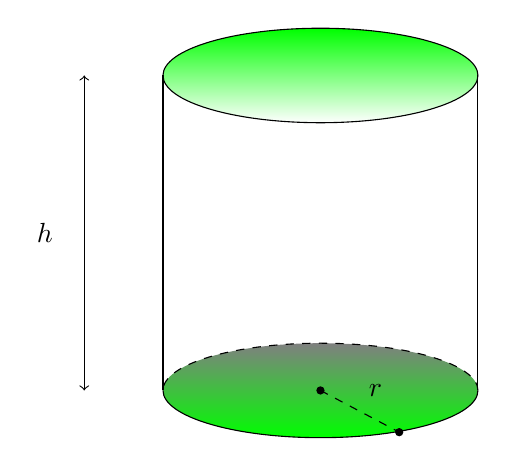
\begin{tikzpicture}[scale=1]
			\shade[top color=green] (0,0) ellipse (2cm and 0.6cm);
			\shade[bottom color=green] (0,-4) ellipse (2cm and 0.6cm);
			\draw (0,0) ellipse (2cm and 0.6cm);
			\draw (-2,0) -- (-2,-4);
			\draw (2,0) -- (2,-4);
			\draw (-2,-4) arc (180:360:2cm and 0.6cm);
			\draw[dashed] (2,-4) arc (0:180:2cm and 0.6cm);
			\fill (0,-4) circle (1.5pt);
			\fill (1,-4.53) circle (1.5pt);
			\draw[dashed] (0,-4) -- (1,-4.53);
			\node at (0.7,-4) {$r$};
			\draw[<->] (-3,0) -- (-3,-4);
			\node at (-3.5,-2) {$h$};
		\end{tikzpicture}
	\end{center}
	\choice
	{$\dfrac{h}{r}=\sqrt{2}$}
	{$\dfrac{h}{r}=2$}
	{\True $\dfrac{h}{r}=6$}
	{$\dfrac{h}{r}=3\sqrt{2}$}
	\loigiai
	{
		Gọi $x$ là giá vật liệu làm mặt xung quanh (cho mỗi đơn vị diện tích).\\
		Thể tích của thùng $V=\pi{r^2}.h$ không đổi. Suy ra $h=\dfrac{V}{\pi{r^2}}.$ (*)\\
		Khi đó, chi phí để làm thùng bằng $P=S_{xq}.x+2S_{\text{đáy}}.3x=2\pi rh.x+2\pi{r^2}.3x=2\pi x\left(3r^2+rh\right)$ .\\
		$\Rightarrow P=2\pi x\left(3r^2+\dfrac{V}{\pi r}\right)=2\pi x\left(3r^2+\dfrac{V}{2\pi r}+\dfrac{V}{2\pi r}\right)\ge 6\pi x.\sqrt[3]{\dfrac{3V^2}{4\pi^2}}.$\\
		$P=6\pi x.\sqrt[3]{\dfrac{3V^2}{4\pi^2}}\Leftrightarrow 3r^2=\dfrac{V}{2\pi r}\Leftrightarrow{r^3}=\dfrac{V}{6\pi}.$\\
		Từ (*) suy ra $\dfrac{h}{r}=\dfrac{V}{\pi{r^3}}=\dfrac{V}{\pi\dfrac{V}{6\pi}}=6$.}
\end{ex}

\begin{ex}%Câu 29 [2H2G1-5]
	Một hình trụ có độ dài đường cao bằng $3$, các đường tròn đáy lần lượt là $\left(O;1\right)$ và $\left(O';1\right)$. Giả sử $AB$ là đường kính cố định của $\left(O;1\right)$ và $CD$ là đường kính thay đổi trên $\left(O';1\right)$. Tìm giá trị lớn nhất $V_{\max}$ của thể tích khối tứ diện $ABCD.$
	\choice
	{\True $V_{\max}=2$}
	{$V_{\max}=6$}
	{$V_{\max}=\dfrac{1}{2}$}
	{$V_{\max}=1$}
	\loigiai
	{\begin{center}
			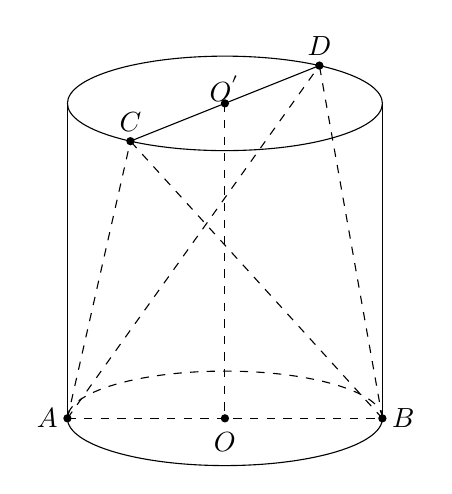
\begin{tikzpicture}[scale=1]
				\draw (0,0) ellipse (2cm and 0.6cm);
				\draw (-2,0) -- (-2,-4);
				\draw (2,0) -- (2,-4);
				\draw (-2,-4) arc (180:360:2cm and 0.6cm);
				\draw[dashed] (2,-4) arc (0:180:2cm and 0.6cm);
				\node[above] at (0,-0.1) {\normalsize$O^{'}$};
				\fill (0,0) circle (1.5pt);
				\node at (0,-4.3) {\normalsize$O$};
				\draw[dashed] (0,0) -- (0,-4);
				\fill (0,-4) circle (1.5pt);
				\fill (-1.2,-0.48) circle (1.5pt);
				\node[above] at (-1.2,-0.48) {\normalsize$C$};
				\fill (1.2,0.48) circle (1.5pt);
				\node[above] at (1.2,0.48) {\normalsize$D$};
				\draw (-1.2,-0.48) -- (1.2,0.48);
				\fill (2,-4) circle (1.5pt);
				\node[right] at (2,-4) {\normalsize$B$};
				\fill (-2,-4) circle (1.5pt);
				\node[left] at (-2,-4) {\normalsize$A$};
				\draw[dashed] (-2,-4) -- (-1.2,-0.48);
				\draw[dashed] (-2,-4) -- (2,-4);
				\draw[dashed] (-2,-4) -- (1.2,0.48);
				\draw[dashed] (2,-4) -- (1.2,0.48);
				\draw[dashed] (2,-4) -- (-1.2,-0.48);
			\end{tikzpicture}
		\end{center}
		Gọi $\alpha $ là số đo góc giữa $AB$ và $CD$.\\
		Ta có $V_{ABCD}=\dfrac{1}{6}AB.CD.\mathrm{\,d}\left(AB,CD\right).\sin\alpha=\dfrac{1}{6}.2.2.3.\sin\alpha=2\sin\alpha\le 2$.\\
		Do đó $V_{ABCD}$ đạt giá trị lớn nhất là $2$, đạt được khi $AB\perp CD$.}
\end{ex}

\begin{ex}%Câu 30 [2H2G1-4]
	Cần sản xuất một vỏ hộp sữa hình trụ có thể tích $V$ cho trước. Để tiết kiệm vật liệu nhất thì bán kính đáy phải bằng
	\choice
	{\True $\sqrt[3]{\dfrac{V}{2\pi}}$}
	{$\sqrt[3]{\dfrac{V}{2}}$}
	{$\sqrt[3]{\dfrac{V}{\pi}}$}
	{$\sqrt[3]{\dfrac{V}{3\pi}}$}
	\loigiai{
		Giả sử vỏ hộp sữa có bán kính đáy là $R$, chiều cao là $h$ ($R,h>0$).\\
		Vì thể tích vỏ hộp là $V$ nên ta có $V=\pi{R^2}h\Rightarrow h=\dfrac{V}{\pi{R^2}}$ .\\
		Để tiết kiệm vật liệu nhất thì hình trụ vỏ hộp sữa phải có diện tích toàn phần\\ $S_{tp}=2\pi Rh+2\pi{R^2}=\dfrac{2V}{R}+2\pi{R^2}$ nhỏ nhất.\\
		\textbf{Cách 1:}\\
		Ta có $S_{tp}=\dfrac{2V}{R}+2\pi{R^2}=\dfrac{V}{R}+\dfrac{V}{R}+2\pi{R^2}\ge 3\sqrt[3]{2\pi{V^2}}$.\\
		$S_{tp}$ đạt giá trị nhỏ nhất khi và chỉ khi $\dfrac{V}{R}=2\pi{R^2}\Leftrightarrow R=\sqrt[3]{\dfrac{V}{2\pi}}$.\\
		\textbf{Cách 2:}\\
		Xét hàm số $f(R)=\dfrac{2V}{R}+2\pi{R^2}$ trên khoảng $\left(0;+\infty\right)$.\\
		Ta có $f'(R)=-\dfrac{2V}{R^2}+4\pi R=\dfrac{4\pi{R^3}-2V}{R^2}$ . $f'(R)=0\Leftrightarrow R=\sqrt[3]{\dfrac{V}{2\pi}}$ .\\
		Bảng biến thiên:\\
		\begin{center}
			\begin{tikzpicture}
				
				\foreach \x [count=\i from 0] in {0,\sqrt[3]{\dfrac{V}{2\pi}},+\infty}% Chỉnh ở đây %i đang 0 đến 4
				{\path (2*\i,0) node {$\x$};\global\let\n=\i} %Gán giá trị n=i, đang là 4
				\foreach \x/\y in {R/0,f'(R)/-1,f(R)/-3}% Chỉnh ở đây
				\path (-1.5,\y) node {$\x$};
				\foreach \x [count=\i from 1] in {-,0,+}
				{\path	 (\i,-1) node {$\x$};}
				\foreach \x/ \y [count=\i from 0] in {/-2,/-4,/-2}% -2 trên, -4 dưới
				{\path	 (2*\i,\y) node(\i) {$\x$};} %node(\i) khai báo 4 điểm đó là (0),...,(3)
				\foreach \x/\y in {0/1,1/2}% Chỉnh ở đây
				\draw[-stealth] (\x)--(\y);%Vẽ dấu mũi tên
				\draw 	(-2.75,0.65) rectangle (2*\n+0.75,-4-0.15) %Vẽ viền xung quanh
				(-2.75,-0.65) rectangle (2*\n+0.75,-1.5)
				(-0.5,0.65)--(-0.5,-4-0.15);%Vẽ đường gạch xuống
			\end{tikzpicture}
		\end{center}
		Từ BBT ta thấy $f(R)$ đạt nhỏ nhất khi $R=\sqrt[3]{\dfrac{V}{2\pi}}$.\\
		Vậy để tiết kiệm vật liệu nhất thì bán kính đáy vỏ hộp phải bằng $\sqrt[3]{\dfrac{V}{2\pi}}$.}
\end{ex}

\begin{ex}%Câu 31 [2H2G1-5]
	Thiết diện của hình trụ và mặt phẳng chứa trục của hình trụ là hình chữ nhật có chu vi là 12$\text{cm}$. Giá trị lớn nhất của thể tích khối trụ là
	\choice
	{$64\pi\,\text{c}{\text{m}^3}$}
	{$16\pi\,\text{c}{\text{m}^3}$}
	{\True $8\pi\,\text{c}{\text{m}^3}$}
	{$32\pi\,\text{c}{\text{m}^3}$}
	\loigiai{
		Gọi chiều cao và bán kính đáy của hình trụ lần lượt là $x$,$y$ $\left(x,\,y>0\,\right)$ .\\
		Khi đó ta có thiết diện của hình trụ và mặt phẳng chứa trục của hình trụ là hình chữ nhật có kích thước lần lượt là $x$ , $2y$.\\
		Theo giả thiết ta có $2.\left(x+2y\right)=12$ $\Leftrightarrow x+2y=6$.\\
		\textbf{Cách 1.}\\
		Thể tích khối trụ: $V=\pi{y^2}.x$ $=\pi{y^2}\left(6-2y\right)=2\pi\left(-y^3+3y^2\right)$ .\\
		Vì $x+2y=6$ $\Rightarrow 0<2y<6\Leftrightarrow 0<y<3.$\\
		Xét hàm số $f(y)=-y^3+3y^2$ trên khoảng $\left(0;3\right)$\\
		Ta có $f'(y)=-3y^2+6y$ $\Rightarrow{f}'(y)=0\Leftrightarrow\left[\begin{aligned}
			& y=0\\ 
			& y=2\\ 
		\end{aligned}\right.$ .\\
		Bảng biến thiên:
		\begin{center}
			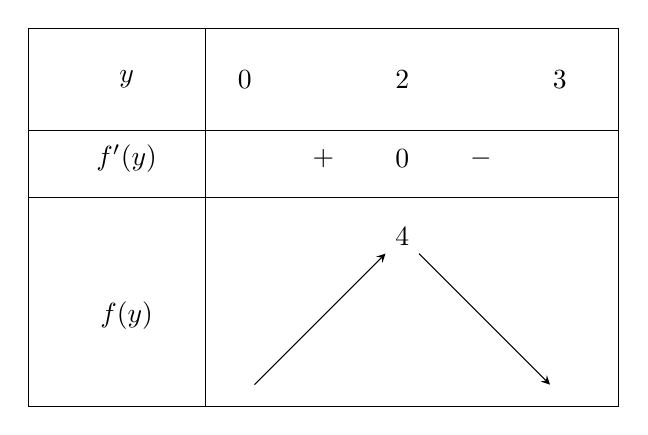
\begin{tikzpicture}
				
				\foreach \x [count=\i from 0] in {0,2,3}% Chỉnh ở đây %i đang 0 đến 4
				{\path (2*\i,0) node {$\x$};\global\let\n=\i} %Gán giá trị n=i, đang là 4
				\foreach \x/\y in {y/0,f'(y)/-1,f(y)/-3}% Chỉnh ở đây
				\path (-1.5,\y) node {$\x$};
				\foreach \x [count=\i from 1] in {+,0,-}
				{\path	 (\i,-1) node {$\x$};}
				\foreach \x/ \y [count=\i from 0] in {/-4,4/-2,/-4}% -2 trên, -4 dưới
				{\path	 (2*\i,\y) node(\i) {$\x$};} %node(\i) khai báo 4 điểm đó là (0),...,(3)
				\foreach \x/\y in {0/1,1/2}% Chỉnh ở đây
				\draw[-stealth] (\x)--(\y);%Vẽ dấu mũi tên
				\draw 	(-2.75,0.65) rectangle (2*\n+0.75,-4-0.15) %Vẽ viền xung quanh
				(-2.75,-0.65) rectangle (2*\n+0.75,-1.5)
				(-0.5,0.65)--(-0.5,-4-0.15);%Vẽ đường gạch xuống
			\end{tikzpicture}
		\end{center}
		Suy ra $\underset{\left(0;3\right)}{\max}\,f(y)=f(2)=4.$\\
		Vậy giá trị lớn nhất của thể tích khối trụ bằng $2\pi .4\,=\,\,8\pi\,\,\text{c}{\text{m}^3}$ .\\
		\textbf{Cách 2.}\\
		Thể tích khối trụ: $V=\pi{y^2}x=\pi .x.y.y\le\pi{\left(\dfrac{x+y+y}{3}\right)^3}=\pi{\left(\dfrac{x+2y}{3}\right)^3}=\pi{\left(\dfrac{6}{3}\right)^3}=8\pi$.\\
		Dấu “=” xảy ra khi $x=y=2$ .\\
		Vậy giá trị lớn nhất của thể tích khối trụ bằng $V=8\pi\,\text{c}{\text{m}^3}.$}
\end{ex}
\begin{ex}%Câu 32 [2H2G1-4]
	Trên một mảnh đất hình vuông có diện tích $81\text{m}^2$ người ta đào một cái ao nuôi cá hình trụ (như hình vẽ) sao cho tâm của hình tròn đáy trùng với tâm của mảnh đất. Ở giữa mép ao và mép mảnh đất người ta để lại một khoảng đất trống để đi lại, biết khoảng cách nhỏ nhất giữa mép ao và mép mảnh đất là $x(\text{m})$. Giả sử chiều sâu của ao cũng là $x(\text{m})$. Tính thể tích lớn nhất V của ao.
	\begin{center}
		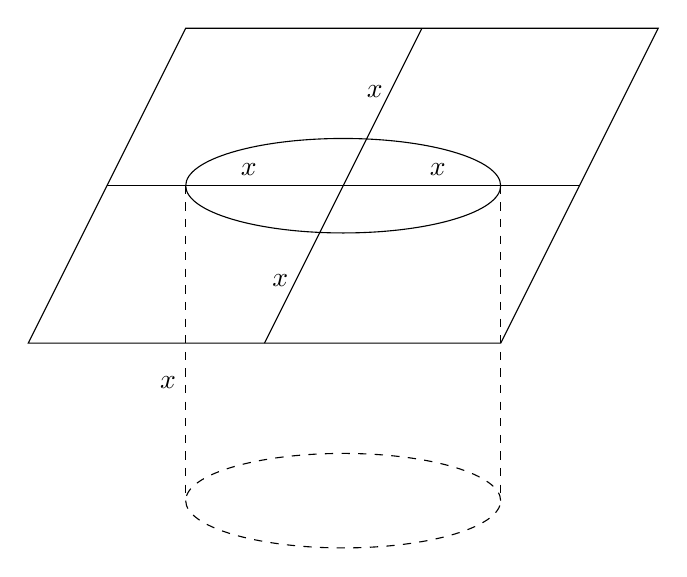
\begin{tikzpicture}[scale=1]
			\draw (-3,0) -- (3,0);
			\draw (1,2) -- (-1,-2);
			\draw (-4,-2) -- (-2,2) -- (4,2) -- (2,-2) -- cycle;
			\draw (0,0) ellipse (2cm and 0.6cm);
			\draw[dashed] (-2,0) -- (-2,-4);
			\draw[dashed] (2,0) -- (2,-4);
			\draw[dashed] (-2,-4) arc (180:360:2cm and 0.6cm);
			\draw[dashed] (2,-4) arc (0:180:2cm and 0.6cm);
			\node at (0.4,1.2) {$x$};
			\node at (-0.8,-1.2) {$x$};
			\node[left] at (-2,-2.5) {$x$};
			\node[above] at (1.2,0) {$x$};
			\node[above] at (-1.2,0) {$x$};
		\end{tikzpicture}
	\end{center}
	\choice
	{\True $V=13,5\pi\left(m^3\right)$}
	{$V=27\pi\left(m^3\right)$}
	{$V=36\pi\left(m^3\right)$}
	{$V=72\pi\left(m^3\right)$}
	\loigiai
	{
		%		\textbf{Phương pháp}\\
		%		Xác định bán kính đáy và chiều cao của hình trụ, sử dụng công thức $V=\pi{R^2}h$ tính thể tích của hình trụ.\\
		%		+) Lập BBT tìm GTLN của hàm thể tích.\\
		%		\textbf{Cách giải}\\
		Ta có: Đường kính đáy của hình trụ là $9-2x\Rightarrow$ Bán kính đáy hình trụ là $\dfrac{9-2x}{2}$ .\\
		Khi đó ta có thể tích ao là $V=\pi{\left(\dfrac{9-2x}{2}\right)^2}x=\dfrac{\pi}{4}{\left(9-2x\right)^2}x=\dfrac{\pi}{4}f(x)$\\
		Xét hàm số $f(x)=\left(9-2x\right)^2x=4x^3-36x^2+81x$ với $0<x<\dfrac{9}{2}$ ta có:\\
		$f'(x)=12x^2-72x+81=0\Leftrightarrow\left[\begin{aligned}
			& x=\dfrac{9}{2}\\ 
			& x=\dfrac{3}{2}\\ 
		\end{aligned}\right.$\\
		BBT:
		\begin{center}
			\begin{tikzpicture}
				
				\foreach \x [count=\i from 0] in {0,\dfrac{3}{2},\dfrac{9}{2}}% Chỉnh ở đây %i đang 0 đến 4
				{\path (2*\i,0) node {$\x$};\global\let\n=\i} %Gán giá trị n=i, đang là 4
				\foreach \x/\y in {x/0,f'(x)/-1,f(x)/-3}% Chỉnh ở đây
				\path (-1.5,\y) node {$\x$};
				\foreach \x [count=\i from 1] in {+,0,-}
				{\path	 (\i,-1) node {$\x$};}
				\foreach \x/ \y [count=\i from 0] in {0/-4,54/-2,0/-4}% -2 trên, -4 dưới
				{\path	 (2*\i,\y) node(\i) {$\x$};} %node(\i) khai báo 4 điểm đó là (0),...,(3)
				\foreach \x/\y in {0/1,1/2}% Chỉnh ở đây
				\draw[-stealth] (\x)--(\y);%Vẽ dấu mũi tên
				\draw 	(-2.75,0.65) rectangle (2*\n+0.75,-4-0.25) %Vẽ viền xung quanh
				(-2.75,-0.65) rectangle (2*\n+0.75,-1.5)
				(-0.5,0.65)--(-0.5,-4-0.25);%Vẽ đường gạch xuống
			\end{tikzpicture}
		\end{center}
		Dựa vào BBT ta thấy $f{(x)_{\max}}=54\Leftrightarrow x=\dfrac{3}{2}$ . Khi đó $V_{\max}=\dfrac{\pi}{4}.54=\dfrac{27\pi}{2}=13,5\pi\left(\text{m}^3\right)$.}
\end{ex}
%%%---34-41
\begin{ex}%[2H2K1-5]%Câu 34	[Chuyên Vĩnh Phúc 2019] 
	Cho hình trụ có đáy là hai đường tròn tâm $O$ và $O'$, bán kính đáy bằng chiều cao và bằng $2a$. Trên đường tròn đáy có tâm $O$ lấy điểm $A$, $D$ sao cho $AD=2\sqrt{3}a$; gọi $C$ là hình chiếu vuông góc của $D$ lên mặt phẳng chứa đường tròn $\left(O'\right)$; trên đường tròn tâm $O'$ lấy điểm $B$ ($AB$ chéo với $CD$). Đặt $\alpha $ là góc giữa $AB$ và đáy. Tính $\tan\alpha $ khi thể tích khối tứ diện $CDAB$ đạt giá trị lớn nhất.
	\choice
	{$\tan\alpha=\sqrt{3}$}
	{$\tan\alpha=\dfrac{1}{\sqrt{2}}$}
	{$\tan\alpha=1$}
	{\True $\tan\alpha=\dfrac{\sqrt{3}}{3}$}
	\loigiai{
		\begin{center}
			\begin{tikzpicture}[line join = round, line cap = round,>=stealth,font=\footnotesize,scale=1]
				\draw[dashed,thin] (-2,0) arc (180:0:2cm and 0.7cm);
				\draw (-2,0) arc (180:360:2cm and 0.7cm) (2,3.5) arc (0:360:2cm and 0.7cm);
				\coordinate (S) at (0,3.5) ;
				\coordinate (M) at (-2,0) ;
				\coordinate (M') at (-2,3.5) ;
				\coordinate (N) at (2,0) ;
				\coordinate (N') at (2,3.5) ;
				\coordinate (O) at (0,0) ;
				\coordinate (O') at (0,3.5) ;
				\coordinate (A) at ($(0,0) + (210:2cm and 0.7cm)$) ;
				\coordinate (D) at ($(0,0) - (135:2cm and 0.7cm)$) ;
				\coordinate (H) at ($(0,0) + (70:2cm and 0.7cm)$) ;
				\coordinate (K) at ($(0,3.5) + (210:2cm and 0.7cm)$) ;
				\coordinate (C) at ($(0,3.5) - (135:2cm and 0.7cm)$) ;
				\coordinate (B) at ($(0,3.5) + (70:2cm and 0.7cm)$) ;
				\draw (M)--(M') (N)--(N') (C)--(B)--(K)--(C)--(D) (A)--(K);
				\draw[dashed] (O)--(O') (H)--(A)--(D)--(H)--(B)--(A);
				\draw pic[draw,angle radius=4mm]{angle=H--A--B};
				\foreach \x/\g in {O/0,O'/60,A/-90,D/-90,H/40,K/90,C/60,B/90}\fill[black](\x)circle(1pt)+(\g:.3)node{$\x$};
			\end{tikzpicture}
			
		\end{center}
		Gọi $H$ là hình chiếu vuông góc của $B$ lên mặt phẳng chứa đường tròn $(O)$ .\\
		Gọi $K$ là hình chiếu vuông góc của $A$ lên mặt phẳng chứa đường tròn $\left(O'\right)$ .\\
		Ta có $HAD.BKC$ là một hình lăng trụ đứng.\\
		Ta có thể tích của tứ diện $CDAB$ là\\
		$V_{ABCD}=\dfrac{1}{3}{V_{HAD.BKC}}=\dfrac{1}{3}\cdot2a\cdot S_{\Delta HAD}=\dfrac{1}{3}\cdot 2a\cdot \dfrac{1}{2}\cdot AD\cdot \left(H;AD\right)=\dfrac{1}{3}\cdot2a\cdot\dfrac{1}{2}\cdot 2a\sqrt{3}\cdot d\left(H;AD\right)$ .\\
		$\left(V_{ABCD}\right)_{\text{max}}\Leftrightarrow{\left(d\left(H;AD\right)\right)_{\text{max}}}$ $\Leftrightarrow $ $H$ là điểm chính giữa cung lớn $\overset\frown{AD}$ của đường tròn $(O)$ (1).\\
		Theo định lý sin ta có $\dfrac{AD}{\sin\widehat{AHD}}=2\cdot2a\Leftrightarrow\sin\widehat{AHD}=\dfrac{AD}{4a}=\dfrac{2\sqrt{3}a}{4a}=\dfrac{\sqrt{3}}{2}$ nên $\widehat{AHD}=60^\circ$.\\
		Do đó (1) xảy ra khi $\Delta AHD$ đều $\Leftrightarrow $ $AH=AD=2\sqrt{3}a$ .\\
		Suy ra $\tan\alpha=\tan\widehat{BAH}=\dfrac{BH}{AH}=\dfrac{2a}{2a\sqrt{3}}=\dfrac{\sqrt{3}}{3}$.}
\end{ex}

\begin{ex}%[2H2K1-5]%Câu 35	[Chuyên Vĩnh Phúc 2019]
	Cho hình trụ có đáy là hai đường tròn tâm $O$ và $O'$, bán kính đáy bằng chiều cao và bằng $2a$. Trên đường tròn đáy có tâm $O$ lấy điểm $A$, $D$ trên đường tròn tâm $O'$ lấy điểm $B$, $C$ sao cho $AB\parallel CD$ và $AB$ không cắt $OO'$. Tính $AD$ để thể tích khối chóp $O'.ABCD$ đạt giá trị lớn nhất.
	\choice
	{\True $AD=2\sqrt{2}a$}
	{$AD=4a$}
	{$AD=\dfrac{4\sqrt{3}}{3}a$}
	{$AD=\sqrt{2}a$}
	\loigiai{
		\begin{center}		\begin{tikzpicture}[line join = round, line cap = round,>=stealth,font=\footnotesize,scale=1]
				\draw[dashed,thin] (-2,0) arc (180:0:2cm and 0.7cm);
				\draw (-2,0) arc (180:360:2cm and 0.7cm) (2,3.5) arc (0:360:2cm and 0.7cm);
				\coordinate (M) at (-2,0) ;
				\coordinate (M') at (-2,3.5) ;
				\coordinate (N) at (2,0) ;
				\coordinate (N') at (2,3.5) ;
				\coordinate (O) at (0,0) ;
				\coordinate (O') at (0,3.5) ;
				\coordinate (A) at ($(0,0) + (210:2cm and 0.7cm)$) ;
				\coordinate (D) at ($(0,0) + (310:2cm and 0.7cm)$) ;
				\coordinate (C) at ($(0,3.5) + (30:2cm and 0.7cm)$) ;
				\coordinate (B) at ($(0,3.5) + (130:2cm and 0.7cm)$) ;
				\coordinate (O1) at ($(A)+(D)-(O)$) ;
				\draw (M)--(M') (N)--(N') (O')--(B)--(C)--(O') (A)--(O1)--(D);
				\draw[dashed] (O)--(O') (B)--(A)--(O')--(O1) (C)--(D)--(O') (O)--(A)--(D)--(O);
				\foreach \x/\g in {O/40,O'/60,A/-90,D/-90,C/60,B/90}\fill[black](\x)circle(1pt)+(\g:.3)node{$\x$};
				\fill (O1) circle(1pt) node[below] {$O_1$};
			\end{tikzpicture}
		\end{center}
		Kẻ đường thẳng qua $O'$ song song với $AB$ cắt mặt phẳng chứa đường tròn $(O)$ tại $O_1$.\\
		Lúc đó $A{O_1}D.BO'C$ là một hình lăng trụ chiều cao bằng $2a$.\\
		Vì $AD=BC$ nên $S_{\Delta BO'C}=S_{\Delta OAD}$\\
		Ta có thể tích của khối chóp $O'.ABCD$:\\
		$V_{O'ABCD}=\dfrac{1}{3}V_{A{O_1}D.BO'C}=\dfrac{2}{3}\cdot 2a\cdot S_{\Delta BO'C}=\dfrac{2}{3}\cdot 2a\cdot S_{\Delta OAD}=\dfrac{2}{3}\cdot2a\cdot\dfrac{1}{2}\cdot2a\cdot2a\cdot\sin\widehat{AOD}\le\dfrac{8a^3}{3}$.\\
		Vậy $V_{O'ABCD}$ đạt giá trị lớn nhất khi $\widehat{AOD}=90^\circ \Leftrightarrow AD =2\sqrt{2}a$.
	}
\end{ex}

\begin{ex}%[2H2K1-5]%Câu 36	[Chuyên Ngoại Ngữ Hà Nội-2021]
	Một hình trụ có thiết diện qua trục là hình chữ nhật có chu vi bằng 12cm. Thể tích lớn nhất mà hình trụ có thể nhận được là
	\choice
	{$16\pi \left(c{m^3}\right)$}
	{$64\pi \left(c{m^3}\right)$}
	{$32\pi \left(c{m^3}\right)$}
	{\True $8\pi \left(c{m^3}\right)$}
	\loigiai{
		\begin{center}
			\begin{tikzpicture}[line join = round, line cap = round,>=stealth,font=\footnotesize,scale=1]
				\draw[dashed,thin] (-2,0) arc (180:0:2cm and 0.7cm);
				\draw (-2,0) arc (180:360:2cm and 0.7cm) (2,3) arc (0:360:2cm and 0.7cm);
				\coordinate (M) at (-2,0) ;
				\coordinate (M') at (-2,3) ;
				\coordinate (N) at (2,0) ;
				\coordinate (N') at (2,3) ;
				\coordinate (O) at (0,0) ;
				\coordinate (O') at (0,3) ;
				\coordinate (C) at ($(0,0) + (30:2cm and 0.7cm)$) ;
				\coordinate (D) at ($(0,0) + (210:2cm and 0.7cm)$) ;
				\coordinate (B) at ($(0,3) + (30:2cm and 0.7cm)$) ;
				\coordinate (A) at ($(0,3) + (210:2cm and 0.7cm)$) ;
				\draw (M)--(M') (N)--(N') (D)--(A)--(B);
				\draw[dashed] (O)--(O') (B)--(C)--(D);
				\foreach \x/\g in {O/-70,O'/60,A/90,D/-90,C/-90,B/90}\fill[black](\x)circle(1pt)+(\g:.3)node{$\x$};
			\end{tikzpicture}
		\end{center}
		Giả sử hình trụ có bán kính đáy là $a$ và chiều cao $h\left(a,h>0\right)$.\\
		Thiết diện qua trục là hình chữ nhật $ABCD$ (như hình vẽ).\\
		Theo giả thiết ta có $2\left(2a+h\right)=12\Leftrightarrow h=6-2a\Rightarrow 0<a<3$ (vì $h>0$).\\
		Thể tích khối trụ là: $V=\pi{a^2}h=\pi{a^2}\left(6-2a\right)=2\pi{a^2}\left(3-a\right)$.\\
		Xét hàm số: $f(a)=a^2\left(3-a\right)\Leftrightarrow f(a)=-a^3+3a^2,\ a\in\left(0;3\right)$.\\
		Có $f'(a)=-3a^2+6a$; $f'(a)=0\Leftrightarrow a=0 \ \ \text{hoặc}\ \ a=2$.\\
		Bảng biến thiên\\
		\begin{center}
			
\begin{tikzpicture}
				\tkzTabInit[nocadre=false,lgt=1.5,espcl=2.5]
				{$a$ /1,$f'(a)$ /1,$f(a)$ /2}{$0$,$2$,$3$}
				\tkzTabLine{,+,$0$,-,}
				\tkzTabVar{-/ $0$,+/ $4$,-/ $0$}
			\end{tikzpicture}
		\end{center}
		Suy ra $\underset{\left(0;3\right)}{\text{max}}\,f(a)=f(2)=4$ .\\
		Vậy $V_{\max}=2\pi \cdot 4=8\pi \left(c{m^3}\right).$
	}
\end{ex}

\begin{ex}%[2H2K1-5]%Câu 37	[THPT Quế Võ 1-Bắc Ninh-2021]
	Cho hình trụ $(T)$ có bán kính đáy và chiều cao đều bằng $R,$ hai đáy là hai hình tròn $(O)$ và $\left(O'\right).$ Gọi $A{A}'$ và $B{B}'$ là hai đường sinh bất kì của $(T)$ và $M$ là một điểm di động trên đường tròn $(O).$ Thể tích lớn nhất của khối chóp $M.A{A}'{B}'B$ bằng bao nhiêu?
	\choice
	{$\dfrac{3R^3\sqrt{3}}{4}$}
	{$\dfrac{R^3\sqrt{3}}{4}$}
	{$\dfrac{R^3\sqrt{3}}{3}$}
	{\True $\dfrac{R^3\sqrt{3}}{2}$}
	\loigiai
	{
		\begin{center}
			\begin{tikzpicture}[line join = round, line cap = round,>=stealth,font=\footnotesize,scale=1]
				\draw[dashed,thin] (-2,0) arc (180:0:2cm and 0.7cm);
				\draw (-2,0) arc (180:360:2cm and 0.7cm) (2,3.5) arc (0:360:2cm and 0.7cm);
				\coordinate (K) at (-2,0) ;
				\coordinate (K') at (-2,3.5) ;
				\coordinate (N) at (2,0) ;
				\coordinate (N') at (2,3.5) ;
				\coordinate (O') at (0,0) ;
				\coordinate (O) at (0,3.5) ;
				\coordinate (A') at ($(0,0) + (40:2cm and 0.7cm)$) ;
				\coordinate (B') at ($(0,0) - (110:2cm and 0.7cm)$) ;
				\coordinate (M) at ($(0,3.5) + (165:2cm and 0.7cm)$) ;
				\coordinate (A) at ($(0,3.5) + (40:2cm and 0.7cm)$) ;
				\coordinate (B) at ($(0,3.5) - (110:2cm and 0.7cm)$) ;
				\coordinate (I) at ($(A)!1/2!(B)$) ;
				\draw (K)--(K') (N)--(N') (M)--(B)--(A)--(M)--(I) (A)--(O)--(B)--(B');
				\draw[dashed] (A')--(M)--(B')--(A')--(A);
				\foreach \x/\g in {O/70,A/90,A'/40,B'/-90,B/-60,I/-30,M/100}\fill[black](\x)circle(1pt)+(\g:.3)node{$\x$};
			\end{tikzpicture}
		\end{center}
		Để tìm giá trị lớn nhất của thể tích của các khối chóp $M.A{A}'{B}'B$ ta chỉ cần xét các loại hình chóp $M.A{A}'{B}'B$ trong đó $M$ là giao điểm của đường tròn $(O)$ và đường trung trực của đoạn $AB.$ Khi đó $O$ thuộc đoạn $MI$ (với $I$ là trung điểm của $AB$).\\
		Đặt $OI=x\,\,\left(0<x<R\right).$\\
		Khi đó $MI=R+x$ và $\left\{\begin{aligned}
			& MI\perp AB\\ 
			& MI\perp A{A}'\\ 
		\end{aligned}\right.\Rightarrow MI\perp\left(A{A}'{B}'B\right).$\\
		Ta có $AB=2AI=2\sqrt{O{A^2}-O{I^2}}=2\sqrt{R^2-x^2}.$\\
		Suy ra thể tích của khối chóp $M.A{A}'{B}'B$ là\\
		$V_{M.A{A}'{B}'B}=\dfrac{1}{3}\cdot\S_{A{A}'{B}'B}\cdot MI=\dfrac{1}{3}.A{A}'\cdot AB\cdot MI=\dfrac{2}{3}R\left(R+x\right)\sqrt{R^2-x^2}.$\\
		$\Rightarrow V_{M.A{A}'{B}'B}^2=\dfrac{4}{9}{R^2}{\left(R+x\right)^2}\left(R^2-x^2\right).$\\
		Áp dụng bất đẳng thức AM-GM, ta có\\
		$\left(R+x\right)^2\left(R^2-x^2\right)=\dfrac{1}{3}\left(R+x\right)\left(R+x\right)\left(R+x\right)\left(3R-3x\right)$\\
		$\le\dfrac{1}{3}{\left(\dfrac{R+x+R+x+R+x+3R-3x}{4}\right)^4}=\dfrac{27R^4}{16}.$\\
		Dấu “$=$ ” xảy ra khi và chỉ khi $\left\{\begin{aligned}
			& R+x=3R-3x\\ 
			& x\in\left(0;R\right)\\ 
		\end{aligned}\right.\Leftrightarrow x=\dfrac{R}{2}.$\\
		Vậy $\text{max} V=\dfrac{2}{3}R\left(R+\dfrac{R}{2}\right)\sqrt{R^2-\left(\dfrac{R}{2}\right)^2}=\dfrac{R^3\sqrt{3}}{2}.$}
\end{ex}

\begin{ex}%[2H2K1-4]%Câu 38	[THPT Phan Đình Phùng-Quảng Bình-2021] 
	Một nhà máy sản xuất các hộp hình trụ kín cả hai đầu có thể tích $V$ cho trước. Mối quan hệ giữa bán kính đáy $R$ và chiều cao $h$ của hình trụ để diện tích toàn phần của hình trụ nhỏ nhất là
	\choice
	{$h=R$}
	{$h=3R$}
	{\True $h=2R$}
	{$R=2h$}
	\loigiai
	{\True\\
		Đặt $R=x$, điều kiện $x>0$.\\
		$V=\pi{x^2}h\Rightarrow h=\dfrac{V}{\pi{x^2}}$ $\Rightarrow\dfrac{h}{R}=\dfrac{V}{\pi{x^3}}$.\\
		$S_{TP}=2\pi R\left(h+R\right)=2\pi x\left(\dfrac{V}{\pi{x^2}}+x\right)=\dfrac{2V}{x}+2\pi{x^2}$.\\
		Xét hàm số: $f(x)=\dfrac{2V}{x}+2\pi{x^2}$ với $x>0$.\\
		Ta có: $f'(x)=-\dfrac{2V}{x^2}+4\pi x=\dfrac{4\pi{x^3}-2V}{x^2}$.\\
		Khi đó: $f'(x)=0\Leftrightarrow x=\sqrt[3]{\dfrac{V}{2\pi}}$.\\
		Ta có bảng biến thiên
		\begin{center}
			
\begin{tikzpicture}
				\tkzTabInit[nocadre=false,lgt=1.5,espcl=2.5]
				{$x$ /1,$f'(x)$ /1,$f(x)$ /2}{$0$,$\sqrt[3]{\frac{V}{2\pi}}$,$+\infty$}
				\tkzTabLine{,-,$0$,+,}
				\tkzTabVar{+/ $+\infty$,-/ $f\left(\sqrt[3]{\frac{V}{2\pi}}\right)$,+/ $+\infty$}
			\end{tikzpicture}
		\end{center}
		Từ BBT trên ta thấy $S_{TP}$ nhỏ nhất khi $x=\sqrt[3]{\dfrac{V}{2\pi}}$.\\
		Khi đó, $\dfrac{h}{R}=\dfrac{V}{\pi\dfrac{V}{2\pi}}=2\Leftrightarrow h=2R$.}
\end{ex}

\begin{ex}%[2H2K1-4]%Câu 39
	Sử dụng mảnh inox hình chữ nhật $ABCD$ có diện tích bằng $1\operatorname{m}^2$ và cạnh $BC=x\left(\operatorname{m}\right)$ để làm một thùng đựng nước có đáy, không có nắp theo quy trình như sau: Chia hình chữ nhật $ABCD$ thành $2$ hình chữ nhật $ADNM$ và $BCNM$, trong đó phần hình chữ nhật $ADNM$ được gò thành phần xung quanh hình trụ có chiều cao bằng $AM$ ; phần hình chữ nhật $BCNM$ được cắt ra một hình tròn để làm đáy của hình trụ trên (phần inox thừa được bỏ đi) Tính gần đúng giá trị $x$ để thùng nước trên có thể tích lớn nhất (coi như các mép nối không đáng kể).\\
	\begin{center}
		\begin{tikzpicture}
			%hinh1
			\draw (0,0) rectangle (4,5);
			\draw (0,2.2) -- (4,2.2);
			\node[below left] at (0,0) {$O$};
			\node[below right] at (4,0) {$C$};
			\node[above left] at (0,5) {$A$};
			\node[above right] at (4,5) {$D$};
			\node[left] at (0,2) {$M$};
			\node[right] at (4,2) {$N$};
			%hinh2
			\draw (8,1) circle (1cm);
			\draw (6,0) rectangle (10,2);
			\node[below left] at (6,0) {$B$};
			\node[below right] at (10,0) {$C$};
			\node[above left] at (6,2) {$M$};
			\node[above right] at (10,2) {$N$};
			%hinh3
		\end{tikzpicture}
		\begin{tikzpicture}[scale=1,line join=round, line cap=round]
			%hinh1
			\def \x{1.8}; %bán kính trục lớn elip
			\def \y{0.8}; %bán kính trục bé elip
			\def \h{3.5}; %chiều cao hình trụ
			\coordinate (A) at (0,0);
			\coordinate (B) at (2*\x,0);
			\coordinate (O) at ($(A)!0.5!(B)$);
			\coordinate (O') at ($(O)+(0,\h)$);
			\coordinate (A') at ($(A)+(0,\h)$);
			\coordinate (B') at ($(B)+(0,\h)$);
			\draw[dashed] (B) arc(0:180:\x cm and \y cm);
			\draw (B) arc(0:-180:\x cm and \y cm);
			\draw (O') ellipse (\x cm and \y cm);
			\tkzDrawSegments(A,A' B,B');
			\tkzDrawSegments[dashed](O,O');
			\tkzDrawSegments[dashed](O,B);
			\tkzDrawSegments(O',B');
			%\tkzLabelSegment(O,B){$r=a$}
			%\tkzLabelSegment[right](B',B){$h=a\sqrt{2}$}
			\tkzDrawPoints[fill=black,size=3](A,B,O,O',A',B');
			%\tkzLabelPoints[left](A,A')
			%\tkzLabelPoints[right](B,B')
			%\tkzLabelPoints[above](O')
			%\tkzLabelPoints[below](O)
		\end{tikzpicture}
		
	\end{center}
	\choice
	{$0{,}97m$}
	{$1{,}37m$}
	{$1{,}12m$}
	{\True $1{,}02m$}
	\loigiai
	{\True\\
		Ta có $AB.BC=1\Rightarrow AB=\dfrac{1}{BC}=\dfrac{1}{x}\left(\operatorname{m}\right)$.\\
		Gọi $r\left(\operatorname{m}\right)$ là bán kính đáy hình trụ inox gò được, ta có chu vi hình tròn đáy bằng $BC=x\left(\operatorname{m}\right).$ Do đó $2\pi r=x\Leftrightarrow r=\dfrac{x}{2\pi}\left(\operatorname{m}\right)$.\\
		Như vậy $BM=2r=\dfrac{x}{\pi}\Rightarrow AM=AB-BM=\dfrac{1}{x}-\dfrac{x}{\pi}\left(\operatorname{m}\right)$.\\
		Thể tích khối trụ inox gò được là $V=\pi{r^2}h=\pi .\left(\dfrac{x}{2\pi}\right)^2.\left(\dfrac{1}{x}-\dfrac{x}{\pi}\right)=\dfrac{1}{4\pi^2}x\left(\pi-x^2\right)$.\\
		Xét hàm số $f(x)=x\left(\pi-x^2\right)$ với $x>0$ .\\
		$f'(x)=\pi-3x^2$; $f'(x)=0\Rightarrow x=\sqrt{\dfrac{\pi}{3}}$;\\
		$f'(x)>0\Leftrightarrow x\in\left(0;\sqrt{\dfrac{\pi}{3}}\right)$ và $f'(x)<0\Leftrightarrow x\in\left(\sqrt{\dfrac{\pi}{3}};+\infty\right)$ .\\
		Bởi vậy $f(x)$ đồng biến trên khoảng $\left(0;\sqrt{\dfrac{\pi}{3}}\right)$ và nghịch biến trên khoảng $\left(\sqrt{\dfrac{\pi}{3}};+\infty\right)$.\\
		Suy ra $\underset{\left(0;+\infty\right)}{\text{max}}\,f(x)=f\left(\sqrt{\dfrac{\pi}{3}}\right)=\dfrac{2\pi\sqrt{3\pi}}{9}$ $\Rightarrow{V_{\text{max}}}\Leftrightarrow f{(x)_{\text{max}}}$ $\Leftrightarrow x=\sqrt{\dfrac{\pi}{3}}\approx 1,02\left(\operatorname{m}\right)$.}
\end{ex}

\begin{ex}%[2H2K1-4]%Câu 40
	Từ một tấm thép phẳng hình chữ nhật, người ta muốn làm một chiếc thùng đựng dầu hình trụ bằng cách cắt ra hai hình tròn bằng nhau và một hình chữ nhật (phần tô đậm) sau đó hàn kín lại, như trong hình vẽ dưới đây. Hai hình tròn làm hai mặt đáy, hình chữ nhật làm thành mặt xung quanh của thùng đựng dầu (vừa đủ). Biết rằng đường tròn đáy ngoại tiếp một tam giác có kích thước là $50cm,\,70cm,\,80cm$ (các mối ghép nối khi gò hàn chiếm diện tích không đáng kể. Lấy $\pi=3{,}14$). Diện tích của tấm thép hình chữ nhật ban đầu gần nhất với số liệu nào sau đây?\\
	\begin{center}
		\begin{tikzpicture}
			\draw (0,0) rectangle (8,4.5);
			\draw (0,1.5) rectangle (8,3); 
			\draw (4,0.75) circle (0.75cm);
			\draw (4,3.75) circle (0.75cm);
			
		\end{tikzpicture}
		\begin{tikzpicture}[scale=1,line join=round, line cap=round]
			%hinh1
			\def \x{1.8} %bán kính trục lớn elip
			\def \y{0.8} %bán kính trục bé elip
			\def \h{3.5} %chiều cao hình trụ
			\coordinate (A) at (0,0);
			\coordinate (B) at (2*\x,0);
			\coordinate (O) at ($(A)!0.5!(B)$);
			\coordinate (O') at ($(O)+(0,\h)$);
			\coordinate (A') at ($(A)+(0,\h)$);
			\coordinate (B') at ($(B)+(0,\h)$);
			\draw[dashed] (B) arc(0:180:\x cm and \y cm);
			\draw (B) arc(0:-180:\x cm and \y cm);
			\draw (O') ellipse (\x cm and \y cm);
			\tkzDrawSegments(A,A' B,B');
			\tkzDrawSegments[dashed](O,O');
			\tkzDrawSegments[dashed](O,B);
			\tkzDrawSegments(O',B');
			
		\end{tikzpicture}
	\end{center}
	\choice
	{$6{,}8$ $\left(\text{m}^{\text{2}}\right)$}
	{$24{,}6$ $\left(\text{m}^{\text{2}}\right)$}
	{\True $6{,}15$ $\left(\text{m}^{\text{2}}\right)$}
	{$3{,}08$ $\left(\text{m}^{\text{2}}\right)$}
	\loigiai
	{\True\\
		Đổi: $50cm=0{,}5m; 70cm=0{,}7m;  80cm=0{,}8m$.\\
		Xét tam giác nội tiếp đường tròn đáy có kích thước lần lượt là $0,5m;\,0,7m;\,0,8m$ nên bán kính đường tròn đáy của thùng đựng dầu là\\
		$R=\dfrac{0,5 \cdot 0,7\cdot 0,8}{4\sqrt{1\left(1-0,5\right)\left(1-0,7\right)\left(1-0,8\right)}}=\dfrac{7\sqrt{3}}{30}$.\\
		Ta có $h=2R$\\
		Diện tích hình chữ nhật ban đầu gấp $3$ lần diện tích xung quanh của hình trụ.\\
		Vậy $S=3\cdot2\pi Rh=6\cdot3,14\cdot2.R^2=6\cdot3,14\cdot2\left(\dfrac{7\sqrt{3}}{30}\right)^2=\dfrac{7693}{1250}=6,1544\,$ $\left(\text{m}^2\right)$.}
\end{ex}

\begin{ex}%[2H2K1-5]%Câu 41 
	[THPT Lê Thánh Tông-HCM-2022] Cho hình trụ tròn xoay có hai đáy là hai hình tròn $\left(I;\sqrt{7}\right)$ và $\left(J;\sqrt{7}\right).$ Biết rằng tồn tại dây cung $EF$ của đường tròn $\left(I;\sqrt{7}\right)$ sao cho tam giác $JEF$ là tam giác đều và mặt phẳng $\left(JEF\right)$ hợp với mặt đáy của hình trụ một góc bằng $60^\circ .$ Thể tích $V$ của khối trụ đã cho là
	\choice
	{\True $V=21\pi $}
	{$V=7\sqrt{6}\pi $}
	{$V=14\pi $}
	{$V=28\pi $}
	\loigiai{
		\begin{center}
			\begin{tikzpicture}
				\draw (0,0) ellipse (2cm and 0.6cm);
				\draw (-2,0) -- (-2,-4);
				\draw (2,0) -- (2,-4);
				\draw (-2,-4) arc (180:360:2cm and 0.6cm);
				\draw[dashed] (2,-4) arc (0:180:2cm and 0.6cm);
				\fill (0,0) circle (1.5pt);
				\fill (0,-4) circle (1.5pt);
				\node[draw,fill,circle,inner sep=1pt,label={-100:$E$}] (E) at (-70:2cm and 0.6cm) {};
				\node[draw,fill,circle,inner sep=1pt,label={90:$F$}] (F) at (45:2cm and 0.6cm) {};
				\draw[dashed] (0,0)--(0,-4);
				\draw[dashed] (-70:2cm and 0.6cm)--(0,-4);
				\draw[dashed] (45:2cm and 0.6cm)--(0,-4);
				\node[above] at (0,0) {$I$};
				\draw (E)--(F);
				\node[below] at (0,-4) {J};
				\fill (2,0) circle (1.5pt);
				\coordinate (H) at ($(E)!0.5!(F)$);
				\node[draw,fill,circle,inner sep=1pt,label={90:$H$}] at (H) {};
				\draw (H) -- (0,0);
				\draw[dashed] (H) -- (0,-4);
			\end{tikzpicture}
		\end{center}
		Gọi $H$ là trung điểm $EF$, có $\widehat{IHJ}=60^\circ.$\\
		Đặt $IJ=h,$ tam giác vuông $JIH$ có $\tan\widehat{JIH}=\dfrac{IJ}{IH}\Leftrightarrow IH=\dfrac{h}{\tan 60^\circ}=\dfrac{h\sqrt{3}}{3}.$, và $\sin\widehat{JHI}=\dfrac{IJ}{JH}\Leftrightarrow JH=\dfrac{h}{\sin 60^\circ}=\dfrac{2h\sqrt{3}}{3}.$\\
		Tam giác đều $JEF$ có $JH=\dfrac{EF\sqrt{3}}{2}\Leftrightarrow EF=\dfrac{2JH}{\sqrt{3}}=2.\dfrac{2h\sqrt{3}}{3\sqrt{3}}=\dfrac{4h}{3}.$\\
		Tam giác vuông $IHE$ có $I{H^2}+H{E^2}=I{E^2}\Leftrightarrow\dfrac{h^2}{3}+\dfrac{4h^2}{9}=7\Leftrightarrow h=3.$\\
		Vậy $V_{(T)}=r^2\cdot\pi \cdot h=7\pi \cdot3=21\pi.$}
\end{ex}
%%%--42-49
\begin{ex}%[2H2G1-1]%Câu 42	[Sở Phú Thọ 2022] 
	Cho hình trụ có bán kính đáy bằng $a\sqrt{3}$. Cắt hình trụ bởi một mặt phẳng song song với trục, cách trục một khoảng bằng $a$ ta được thiết diện là một hình vuông. Thể tích khối trụ đó bằng
	\choice
	{$2\pi a^3\sqrt{2}$}
	{$4\pi a^3\sqrt{2}$}
	{\True $6\pi a^3\sqrt{2}$}
	{$3\pi a^3\sqrt{2}$}
	\loigiai{
		\immini{
			Dựng $OI\perp AB$ khi đó $I$ là trung điểm $AB$.\\
			Ta có $IA=\sqrt{OA^2-IO^2}=\sqrt{3a^2-a^2}=a\sqrt{2}$.\\
			Vì $ABCD$ là hình vuông nên $AB=2a\sqrt{2}$.\\
			Thế tích hình trụ $V=\pi R^2h=6\pi a^3\sqrt{2}\,\left(\text{đvtt}\right)$.
		}{
			\begin{tikzpicture}[line join = round, line cap = round,>=stealth,font=\footnotesize,scale=0.8]
				\draw[dashed,thin] (2.5,0) arc (0:180:2.5cm and 0.7cm);
				\draw (2.5,4) arc (0:360:2.5cm and 0.7cm) (-2.5,0) arc (180:360:2.5cm and 0.7cm);
				\coordinate (O') at (0,4);
				\coordinate (O) at (0,0);
				\coordinate (M) at (-2.5,0);
				\coordinate (N) at (2.5,0);
				\coordinate (M') at (-2.5,4);
				\coordinate (N') at (2.5,4);
				\coordinate (A) at ($(0,0) - (110:2.5cm and 0.7cm)$) ;
				\coordinate (B) at ($(0,0) + (45:2.5cm and 0.7cm)$) ;
				\coordinate (D) at ($(0,4) - (110:2.5cm and 0.7cm)$) ;
				\coordinate (C) at ($(0,4) + (45:2.5cm and 0.7cm)$) ;
				\coordinate (I) at ($(A)!1/2!(B)$);
				\draw (M)--(M') (N)--(N') (A)--(D)--(C);
				\draw[dashed] (A)--(B)--(C) (O)--(O') (I)--(O)--(A);
				\foreach \x/\g in {A/-130,B/30,C/90,D/120,O/180,O'/180,I/-30}\fill[black](\x)circle(1pt)+(\g:.3)node{$\x$} ;
			\end{tikzpicture}
		}
	}
\end{ex}

\begin{ex}%[2H2G1-1]%Câu 43	[Chuyên Hạ Long 2022]
	Cho hình trụ tròn xoay có hai đáy là hai hình tròn $(O ; R)$ và $\left(O' ; R\right)$. Tồn tại dây cung $A B$ thuộc đường tròn $(O)$ sao cho $\Delta O' A B$ là tam giác đều và mặt phẳng $\left(O' A B\right)$ hợp với mặt phẳng chứa đường tròn $(O)$ một góc $60^\circ$. Khi đó diện tích xung quanh $S_{x q}$ hình trụ là
	\choice
	{$S_{x q}=\dfrac{4\pi R^2}{7}$}
	{$S_{x q}=\dfrac{3\pi R^2}{\sqrt{7}}$}
	{$S_{x q}=\dfrac{3\pi R^2\sqrt{7}}{7}$}
	{\True $S_{x q}=\dfrac{6\pi R^2\sqrt{7}}{7}$}
	\loigiai{
		\immini{
			Gọi $I$ là trung điểm $A B$. Khi đó $O I\perp A B$.\\
			Xét tam giác $O' O I$ vuông tại $O$ có 
			$$O I=\dfrac{O' O}{\tan 60^\circ}=\dfrac{O' O}{\sqrt{3}} \text{ và } O' I=\dfrac{O' O}{\sin 60^\circ}=\dfrac{2 O' O}{\sqrt{3}}.$$ 
			Mặt khác xét $\triangle OIA$ vuông tại $I$ có $$A I^2=R^2-O I^2=R^2-\dfrac{O O'^{2}}{3}\Rightarrow A B^2=4\left(R^2-\dfrac{O' O^2}{3}\right).$$
			Vì $\triangle O' A B$ đều nên $O' I=A B\dfrac{\sqrt{3}}{2}$
			$$\Leftrightarrow O' I^2=\dfrac{3}{4}A B^2\Leftrightarrow\dfrac{4}{3}O' O^2=3 R^2-O' O^2\Leftrightarrow O' O=\dfrac{3 R}{\sqrt{7}}.$$
			Diện tích xung quanh hình trụ $S_{x q}=2\pi R\cdot O' O=\dfrac{6\pi R^2\sqrt{7}}{7}$.
		}{
			\begin{tikzpicture}[line join = round, line cap = round,>=stealth,font=\footnotesize,scale=0.8]
				\draw[dashed,thin] (2.5,0) arc (0:180:2.5cm and 0.7cm);
				\draw (2.5,4) arc (0:360:2.5cm and 0.7cm) (-2.5,0) arc (180:360:2.5cm and 0.7cm);
				\coordinate (O') at (0,4);
				\coordinate (O) at (0,0);
				\coordinate (M) at (-2.5,0);
				\coordinate (N) at (2.5,0);
				\coordinate (M') at (-2.5,4);
				\coordinate (N') at (2.5,4);
				\coordinate (A) at ($(0,0) - (110:2.5cm and 0.7cm)$) ;
				\coordinate (B) at ($(0,0) + (45:2.5cm and 0.7cm)$) ;
				\coordinate (I) at ($(A)!1/2!(B)$);
				\draw (M)--(M') (N)--(N');
				\draw[dashed] (O')--(A)--(B)--(O')--(O)--(I)--(O');
				\foreach \x/\g in {A/-130,B/30,O/180,O'/180,I/-30}\fill[black](\x)circle(1pt)+(\g:.3)node{$\x$} ;
			\end{tikzpicture}
		}
	}
\end{ex}

\begin{ex}%[2H2G1-1]%Câu 44	[THPT Kim Liên-Hà Nội-2022]
	Cắt hình trụ $(T)$ có bán kính $R$ bởi một mặt phẳng song song với trục và cách trục một khoảng bằng $a\,\left(0<a<R\right)$ ta được thiết diện là một hình vuông có diện tích $16a^2$. Diện tích xung quanh của hình trụ $(T)$ bằng
	\choice
	{$4\pi{a^2}\sqrt{5}$}
	{$\pi{a^2}\sqrt{5}$}
	{\True $8\pi{a^2}\sqrt{5}$}
	{$16\pi{a^2}\sqrt{5}$}
	\loigiai{
		\immini{
			Hình trụ có hai tâm của hai đường tròn đáy là $O_1,\,O_2$. Mặt phẳng thiết diện là hình vuông $ABCD$.\\
			Hình vuông $ABCD$ có diện tích là $16a^2$ nên cạnh $AB=BC=4a$.\\
			Gọi $I$ là trung điểm của $AB$, suy ra $IB=\dfrac{AB}{2}=2a$.\\
			Mặt khác, khoảng cách từ $O_1O_2$ đến $(ABCD)$ là $a$ nên $O_1I=a$.\\
			Tam giác $O_1IB$ vuông tại $I$ nên 
			$$R=O_1B=\sqrt{O_1I^2+IB^2}=\sqrt{a^2+\left(2a\right)^2}=a\sqrt{5}.$$
			Diện tích xung quanh hình trụ $(T)$ là 
			$$S_{xq}=2\pi Rh=2\pi\cdot R\cdot BC=2\pi\cdot a\sqrt{5}\cdot 4a=8a^2\pi\sqrt{5}.$$
		}{
			\begin{tikzpicture}[line join = round, line cap = round,>=stealth,font=\footnotesize,scale=0.8]
				\draw[dashed,thin] (2.5,0) arc (0:180:2.5cm and 0.7cm);
				\draw (2.5,4) arc (0:360:2.5cm and 0.7cm) (-2.5,0) arc (180:360:2.5cm and 0.7cm);
				\coordinate (O') at (0,4) ;
				\coordinate (O) at (0,0) ;
				\coordinate (M) at (-2.5,0);
				\coordinate (N) at (2.5,0);
				\coordinate (M') at (-2.5,4);
				\coordinate (N') at (2.5,4);
				\coordinate (A) at ($(0,0) - (110:2.5cm and 0.7cm)$) ;
				\coordinate (B) at ($(0,0) + (45:2.5cm and 0.7cm)$) ;
				\coordinate (D) at ($(0,4) - (110:2.5cm and 0.7cm)$) ;
				\coordinate (C) at ($(0,4) + (45:2.5cm and 0.7cm)$) ;
				\coordinate (I) at ($(A)!1/2!(B)$);
				\draw (M)--(M') (N)--(N') (A)--(D)--(C);
				\draw[dashed] (A)--(B)--(C) (B)--(O)--(O') (I)--(O)--(A);
				\foreach \x/\g in {A/-130,B/30,C/90,D/120,I/-30}\fill[black](\x)circle(1pt)+(\g:.3)node{$\x$} ;
				\fill (O) circle(1pt) node [left] {$O_1$} (O') circle(1pt) node [left] {$O_2$};
			\end{tikzpicture}
		}
	}
\end{ex}

\begin{ex}%[2H2G1-1]%Câu 45	[THPT Yên Lạc-Vĩnh Phúc-2022]
	Cho hình trụ $(T)$ chiều cao bằng $2a$, hai đường tròn đáy của $(T)$ có tâm lần lượt là $O$ và $O_1$, bán kính bằng $a$. Trên đường tròn đáy tâm $O$ lấy điểm $A$, trên đường tròn đáy tâm $O_1$ lấy điểm $B$ sao cho $AB=\sqrt{5}a$. Thể tích khối tứ diện $OO_1AB$ bằng
	\choice
	{$\dfrac{\sqrt{3} a^3}{12}$}
	{$\dfrac{\sqrt{3} a^3}{3}$}
	{$\dfrac{\sqrt{3} a^3}{4}$}
	{\True $\dfrac{\sqrt{3} a^3}{6}$}
	\loigiai{
		\immini{
			Gọi $C$ là điểm trên đường tròn tâm $O$ sao cho $BC \parallel OO_1$. Khi đó tứ giác $OCBO_1$ là hình chữ nhật và có diện tích là $S_{OCBO_1}=2a^2$.\\
			Xét $\triangle ABC$ vuông, có $AC=\sqrt{AB^2-BC^2}=a$ nên $\triangle OAC$ đều.\\
			Gọi $H$ là trung điểm của $OC$, ta có $AH\perp OC$ và $AH=\dfrac{a\sqrt{3}}{2}$.\\
			Mặt khác $\left(ACO\right)\perp\left(OCBO_1\right)$ nên $AH\perp\left(OCBO_1\right)$.\\
			Thể tích khối chóp $A.OCBO_1$ là 
			$$V_{A.OCBO_1}=\dfrac{1}{3}AH\cdot S_{O.ACBO_1}=\dfrac{a^3\sqrt{3}}{3}.$$
			Thể tích khối tứ diện $OO_1AB$ bằng thể tích khối chóp $A.OBO_1$ 
			$$\Rightarrow V_{AOBO_1}=\dfrac{1}{2} V_{A.OCBO_1}=\dfrac{a^3\sqrt{3}}{6}.$$
		}{
			\begin{tikzpicture}[line join = round, line cap = round,>=stealth,font=\footnotesize,scale=0.8]
				\draw[dashed,thin] (2.5,0) arc (0:180:2.5cm and 0.7cm);
				\draw (2.5,4) arc (0:360:2.5cm and 0.7cm) (-2.5,0) arc (180:360:2.5cm and 0.7cm);
				\coordinate (O') at (0,4) ;
				\coordinate (O) at (0,0) ;
				\coordinate (M) at (-2.5,0);
				\coordinate (N) at (2.5,0);
				\coordinate (M') at (-2.5,4);
				\coordinate (N') at (2.5,4);
				\coordinate (C) at ($(0,0) - (140:2.5cm and 0.7cm)$) ;
				\coordinate (B) at ($(0,4) - (140:2.5cm and 0.7cm)$) ;
				\coordinate (A) at ($(0,0) - (60:2.5cm and 0.7cm)$) ;
				\coordinate (H) at ($(O)!1/2!(C)$);
				\draw (M)--(M') (N)--(N') (O')--(B)--(C);
				\draw[dashed] (A)--(B)--(O)--(A)--(O')--(O) (B)--(O)--(C)--(A)--(H);
				\foreach \x/\g in {A/-130,B/90,C/-90,H/70,O/160}\fill[black](\x)circle(1pt)+(\g:.3)node{$\x$} ;
				\fill (O') circle(1pt) node [left] {$O_1$};
			\end{tikzpicture}
		}
	}
\end{ex}

\begin{ex}%[2H2G1-1]%Câu 46	[Sở Nam Định 2022] 
	\immini{
		Cho hình trụ $(T)$ có hai đáy là hai hình tròn $(O);\left(O'\right)$ và thiết diện qua trục của hình trụ là hình vuông. Điểm $A$ thuộc đường tròn $(O)$, điểm $B$ thuộc đường tròn $\left(O'\right)$ sao cho $AB=2$ và khoảng cách giữa $AB$ và $OO'$ bằng $\dfrac{\sqrt{3}}{2}$ (thao khảo hình bên). Khối trụ $(T)$ có thể tích bằng
		\choice
		{$\dfrac{7\sqrt{14}}{8}\pi $}
		{$\dfrac{7\sqrt{14}}{2}\pi $}
		{$\dfrac{28\sqrt{14}}{27}\pi $}
		{\True $\dfrac{7\sqrt{14}}{16}\pi $}
	}{
		\begin{tikzpicture}[line join = round, line cap = round,>=stealth,font=\footnotesize,scale=0.8]
			\draw[dashed,thin] (2.5,0) arc (0:180:2.5cm and 0.7cm);
			\draw (2.5,4) arc (0:360:2.5cm and 0.7cm) (-2.5,0) arc (180:360:2.5cm and 0.7cm);
			\coordinate (O) at (0,4) ;
			\coordinate (O') at (0,0) ;
			\coordinate (C) at (-2.5,0);
			\coordinate (N) at (2.5,0);
			\coordinate (A) at (-2.5,4);
			\coordinate (N') at (2.5,4);
			\coordinate (B) at ($(0,0) - (70:2.5cm and 0.7cm)$) ;
			\coordinate (H) at ($(O)!1/2!(C)$);
			\draw (A)--(C) (N)--(N') (O)--(A);
			\draw[dashed] (A)--(B)--(O')--(O) (O')--(C);
			\foreach \x/\g in {A/130,B/-90,O/90,O'/-20}\fill[black](\x)circle(1pt)+(\g:.3)node{$\x$} ;
		\end{tikzpicture}
	}
	\loigiai{
		\immini{
			Dựng $AC \parallel OO'$, $O'I \perp CB$.\\
			Ta có $\heva{&O'I\perp CB\\ &O'I\perp AC} \Rightarrow O'I\perp\left(ACB\right)$
			$$\Rightarrow d\left(OO',AB\right)=d\left(O',\left(ABC\right)\right)=O'I=\dfrac{\sqrt{3}}{2}.$$
			Gọi $OO'=2x,\,\left(x>0\right)$.\\
			Khi đó $IB=\sqrt{O'B^2-O'I^2}=\sqrt{x^2-\dfrac{3}{4}}$
			$$\Rightarrow CB=2IB=2\sqrt{x^2-\dfrac{3}{4}}.$$
			Mà $AC=OO'=2x \Rightarrow AC=\sqrt{4-4\left(x^2-\dfrac{3}{4}\right)}=2x$\\
			$$\Leftrightarrow 4x^2=7-4x^2\Leftrightarrow x=\pm\sqrt{\dfrac{7}{8}} \text{ vì } x>0 \text{ nên } x=\sqrt{\dfrac{7}{8}}.$$
			Thể tích khối lăng trụ $V=\pi r^2\cdot h=\pi \cdot\dfrac{7}{8}\cdot 2\dfrac{\sqrt{7}}{\sqrt{8}}=\dfrac{7\sqrt{14}\pi}{16}$.
		}{
			\begin{tikzpicture}[line join = round, line cap = round,>=stealth,font=\footnotesize,scale=0.8]
				\draw[dashed,thin] (2.5,0) arc (0:180:2.5cm and 0.7cm);
				\draw (2.5,4) arc (0:360:2.5cm and 0.7cm) (-2.5,0) arc (180:360:2.5cm and 0.7cm);
				\coordinate (O) at (0,4) ;
				\coordinate (O') at (0,0) ;
				\coordinate (C) at (-2.5,0);
				\coordinate (N) at (2.5,0);
				\coordinate (A) at (-2.5,4);
				\coordinate (N') at (2.5,4);
				\coordinate (B) at ($(0,0) - (70:2.5cm and 0.7cm)$) ;
				\coordinate (I) at ($(B)!1/2!(C)$);
				\draw (A)--(C) (N)--(N') (O)--(A);
				\draw[dashed] (A)--(B)--(O')--(O) (O')--(C)--(B) (A)--(I)--(O');
				\foreach \x/\g in {A/130,B/-90,C/-150,O/90,O'/-20,I/-90}\fill[black](\x)circle(1pt)+(\g:.3)node{$\x$} ;
			\end{tikzpicture}
		}
	}
\end{ex}

\begin{ex}%[2H2G1-1]%Câu 47	[THPT Phụ Dực-Quảng Bình 2022]
	Cho hình trụ có đường kính đáy bằng $\sqrt{5}$. Hình vuông $A B C D$ nội tiếp hình trụ với hai điểm $A, B$ thuộc đường tròn là đáy trên và $C, D$ thuộc đường tròn đáy dưới của hình trụ và $A B<3$. Biết diện tích hình chiếu của hình vuông $A B C D$ trên mặt đáy bằng $2$ (đơn vị diện tích). Tính thể tích của khối trụ đó.
	\choice
	{$\dfrac{5\pi\sqrt{3}}{12}$}
	{$\dfrac{5\pi\sqrt{6}}{6}$}
	{$\dfrac{5\pi\sqrt{6}}{2}$}
	{\True $\dfrac{5\pi\sqrt{3}}{4}$}
	\loigiai{
		\immini{
			Ta kẻ lần lượt các đường sinh $CC'$ và $DD'$ với $C',\, D'\in\left(O ;\dfrac{\sqrt{5}}{2}\right)$ sao cho $S_{A B C' D'}=2$.\\
			Khi đó $A B C' D'$ là hình chữ nhật, ta có $S_{A B C' D'}=A B\cdot B C'=2$.\\
			Mà $A B^2+B C'^{2}=(2 R)^2=5$ nên ta có hệ phương trình sau 
			$$\heva{&AB\cdot BC'=2\\ &AB^2+BC'^2=5.}$$
			Do $A B<3$ nên hệ phương trình có nghiệm 
			$$\heva{&A B=B C=1\\ &B C'=2} \text{ hoặc } \heva{&A B=B C=2\\ &B C'=1.}$$
		}{
			\begin{tikzpicture}[line join = round, line cap = round,>=stealth,font=\footnotesize,scale=0.8]
				\draw[dashed,thin] (2.5,0) arc (0:180:2.5cm and 0.7cm);
				\draw (2.5,4) arc (0:360:2.5cm and 0.7cm) (-2.5,0) arc (180:360:2.5cm and 0.7cm);
				\coordinate (O') at (0,4) ;
				\coordinate (O) at (0,0) ;
				\coordinate (A) at (-2.5,0);
				\coordinate (C') at (2.5,0);
				\coordinate (M') at (-2.5,4);
				\coordinate (C) at (2.5,4);
				\coordinate (B) at ($(0,0) - (110:2.5cm and 0.7cm)$) ;
				\coordinate (D') at ($(0,0) + (110:2.5cm and 0.7cm)$) ;
				\coordinate (D) at ($(0,4) + (110:2.5cm and 0.7cm)$) ;
				\coordinate (I) at ($(O)!1/2!(O')$);
				\coordinate (H) at ($(A)!1/2!(B)$);
				\draw (A)--(M') (D)--(C)--(C') ;
				\draw[dashed] (B)--(D')--(D)--(A)--(B)--(C) (C')--(A)--(C)--(B) (A)--(D')--(C')--(B) (O)--(O') (I)--(H)--(O);
				\foreach \x/\g in {A/-130,C/40,C'/-40,B/-90,D'/50,D/90,O/50,O'/20,I/140,H/-110}\fill[black](\x)circle(1pt)+(\g:.3)node{$\x$} ;
			\end{tikzpicture}
		}
		\noindent \textbf{Trường hợp 1:} $\heva{&A B=B C=1\\ &B C'=2}\Rightarrow C C'=h=\sqrt{B C^2-B C'^2}$ không tồn tại nên loại.\\
		\textbf{Trường hợp 2:} $\heva{&A B=B C=2\\ &B C'=1}\Rightarrow C C'=h=\sqrt{B C^2-B C'^2}=\sqrt{3}$.\\
		Vậy ta suy ra thể tích khối trụ là $V=\pi R^2h=\pi\left(\dfrac{\sqrt{5}}{2}\right)^2\sqrt{3}=\dfrac{5\pi\sqrt{3}}{4}$.
	}
\end{ex}

\begin{ex}%[2H2G1-4]%Câu 48	[Sở Nghệ An 2022] 
	Ống thép mạ kẽm (độ dày ống thép là hiệu số bán kính mặt ngoài và bán kính mặt bên trong của ống thép). Nhà máy quy định giá bán cho các ống thép dựa trên cân nặng của các ống thép đó. Biết rằng thép ống có giá $24700$ đồng/kg và khối lượng riêng của thép là $7850~kg/{m}^3$. Một đại lý thép mua về $1000$ ống loại có đường kính ống ngoài là $108~mm$, độ dày là $3~mm$ và có chiều dài $6~m$. Hãy tính số tiền mà đại lí bỏ ra để mua $1000$ ống thép nói trên (làm tròn đến ngàn đồng).
	%	\begin{center}
		%%		\includegraphics{H1.png}
		%	\end{center}
	\choice
	{\True 1151273000}
	{1113789000}
	{1223867000}
	{1124980000}
	\loigiai{
		Vì độ dày ống thép là hiệu số bán kính mặt ngoài và bán kính mặt bên trong của ống thép nên ta có thể tích thép của mỗi ống bằng 
		\begin{eqnarray*}
			\pi\left(r_1^2-r_2^2\right)\cdot h &=& \pi\left(0{,}054^2-0{,}051^2\right)\cdot 6\,\left(m^3\right)\\
			&=& \pi\cdot 1{,}89\cdot 10^{-3}\,\left(m^3\right).
		\end{eqnarray*}
		Trong đó $r_1,\, r_2$ lần lượt là bán kính ống ngoài và trong).\\
		Vậy số tiền phải trả để mua $1000$ ống thép nói trên là
		$$\pi\cdot 1{,}89\cdot{10^{-3}}\cdot 1000\cdot 7850\cdot 24700 \approx 1151272913 \approx 1151273000\text{ (đồng).}$$
	}
\end{ex}

\begin{ex}%[2H2G1-1]%Câu 49	[Chuyên ĐHSP Hà Nội 2022] 
	Cho hình trụ có hai đáy là hai hình tròn $\left(O;R\right)$ và $\left(O';R\right)$. Gọi $AB$ là một dây cung của đường tròn $\left(O;R\right)$ sao cho tam giác $O'AB$ là tam giác đều và mặt phẳng $\left(O'AB\right)$ tạo với mặt phẳng chứa đường tròn $\left(O;R\right)$ một góc $60^\circ $. Tính theo $R$ thể tích $V$ của khối trụ đã cho
	\choice
	{$V=\dfrac{3\pi\sqrt{5} R^3}{5}$}
	{$V=\dfrac{\pi\sqrt{7} R^3}{7}$}
	{\True $V=\dfrac{3\pi\sqrt{7} R^3}{7}$}
	{$V=\dfrac{\pi\sqrt{5} R^3}{5}$}
	\loigiai{
		\immini{
			Gọi $K$ là trung điểm $AB$, đặt $AB=2a$.\\
			Ta có $AB\perp OK$ và $AB\perp O{O}'$ nên 
			\begin{eqnarray*}
				\widehat{OKO'}=60^\circ &\Rightarrow& O'K=2OK\\
				&\Rightarrow& O'K^2=4OK^2\\
				&\Rightarrow& 3a^2=4\left(R^2-a^2\right)\\
				&\Rightarrow& a^2=\dfrac{4R^2}{7}.
			\end{eqnarray*}
		}{
			\begin{tikzpicture}[line join = round, line cap = round,>=stealth,font=\footnotesize,scale=0.8]
				\draw[dashed,thin] (2.5,0) arc (0:180:2.5cm and 0.7cm);
				\draw (2.5,4) arc (0:360:2.5cm and 0.7cm) (-2.5,0) arc (180:360:2.5cm and 0.7cm);
				\coordinate (O') at (0,4);
				\coordinate (O) at (0,0);
				\coordinate (M) at (-2.5,0);
				\coordinate (N) at (2.5,0);
				\coordinate (M') at (-2.5,4);
				\coordinate (N') at (2.5,4);
				\coordinate (A) at ($(0,0) - (110:2.5cm and 0.7cm)$) ;
				\coordinate (B) at ($(0,0) + (45:2.5cm and 0.7cm)$) ;
				\coordinate (K) at ($(A)!1/2!(B)$);
				\draw (M)--(M') (N)--(N');
				\draw[dashed] (O')--(A)--(B)--(O')--(O)--(K)--(O');
				\foreach \x/\g in {A/-130,B/30,O/180,O'/180,K/-30}\fill[black](\x)circle(1pt)+(\g:.3)node{$\x$} ;
			\end{tikzpicture}
		}
		\noindent Mặt khác $OO'^2=O'B^2-OB^2=4a^2-R^2=4\cdot\dfrac{4R^2}{7}-R^2=\dfrac{9R^2}{7} \Rightarrow O'O=\dfrac{3\sqrt{7}R}{7}$.\\
		Vậy thể tích khối trụ là $V=\pi R^2h=\dfrac{3\pi\sqrt{7} R^3}{7}$.
	}
\end{ex}
\Closesolutionfile{ans}
\indapan{10}{ans/CD22/Muc_9_10}